\documentclass[lang=cn,10pt]{elegantbook}

\title{智弈锋穹——AI驱动的攻防自治演训靶场}
\subtitle{项目文档}

\author{何树贤、易梦哲、周君赢、陈易东、张军、牟航、周望、张顾峰、黄睿哲、孙明皓}
\bioinfo{指导老师}{张立强、何艺、严飞}
\institute{武汉大学 国家网络安全学院}
\date{2025年8月14日}


\setcounter{tocdepth}{3}

% \logo{cyber-4084719_1280.jpg}
\cover{cyber-4084719_1280.jpg}


% 本文档命令
\usepackage{graphicx}  % 插入图片的宏包
\usepackage{caption}   % 自定义标题
\usepackage{array}
\usepackage{hyperref}
\usepackage{tcolorbox}
\newcommand{\ccr}[1]{\makecell{{\color{#1}\rule{1cm}{1cm}}}}
\usepackage{listings}
\usepackage{xcolor} % 支持颜色

\lstset{
    basicstyle=\ttfamily\small,  % 等宽字体,字号
    backgroundcolor=\color{gray!10}, % 浅灰背景
    frame=single,                % 单线边框
    rulecolor=\color{black!30},  % 边框颜色
    breaklines=true,             % 自动换行
    postbreak=\mbox{$\hookrightarrow$}, % 换行标记
    keywordstyle=\color{blue},   % 关键字高亮
    commentstyle=\color{green!50!black}, % 注释颜色
    stringstyle=\color{red},     % 字符串颜色
    showstringspaces=false       % 不显示字符串中的空格
}

% 修改标题页的橙色带
\definecolor{customcolor}{RGB}{7,8,8}
\colorlet{coverlinecolor}{customcolor}

\begin{document}

% \begin{figure}[H]
% \centering
% \includegraphics[width=0.7\textwidth]{your_image_path_here}  % 将路径替换为图片的路径
% \caption{这是第一张图片的标题}  % 图片的标题,可编辑
% \label{fig:fig1}  % 标签,用于引用
% \end{figure}

\maketitle
\frontmatter

\tableofcontents

\mainmatter


\chapter{项目背景和概述}
\begin{introduction}
    \item 赛题背景
    \item 基本知识背景
\end{introduction}

\section{赛题背景}

党的十八大以来,以习近平同志为核心的党中央高度重视网络安全工作,特别在目前日趋复杂
的背景下,深刻认识和有力防范网络安全风险,切实维护网络空间安全,已成为事关全局的重大课
题。

\begin{figure}[htbp]
\centering

\includegraphics[width=0.7\textwidth]{cybersecurity.png}  % 将路径替换为图片的路径
\caption{网络安全}  % 图片的标题,可编辑
\label{fig:网络安全}  % 标签,用于引用
\end{figure}

随着《网络安全法》和《国家网络空间安全战略》的深入推进,
实战化网络攻防能力的建设成为网络安全体系中的关键任务之一,
尤其在“十五五”规划对关键信息基础设施安全防护提出更高要求的背景下,
传统的网络安全演练方式已难以满足动态演训和智能对抗的发展趋势,
目前在实际操作中面临三方面的主要瓶颈:

\textbf{一是传统靶场场景构建模式过于静态},往往采用人工预设的方式搭建演练环境,
更新周期长、调整代价高,导致其难以及时引入现实世界中快速变化的业务架构、
操作流程以及技术组件,也无法涵盖近年来不断涌现的新型攻击方式与复杂威胁模型,
例如\textbf{APT、供应链渗透}等,这种脱节使得演练内容始终滞后于现实威胁的发展态势,
无法为参与者提供贴近实战的演练体验,也难以检验系统和人员在面对未知攻击时的应对能力,
从而削弱了靶场演练在实战能力培养中的实际价值。

\textbf{二是攻击路径往往依赖人工预设},主要根据经验规则构建固定的攻击链条,
缺乏动态生成机制与策略调整能力,导致攻击行为表现出明显的模式化特征,
不仅在路径选择上缺乏多样性,也难以模拟出真实渗透过程中攻击者面对防护机制时的适应性调整与策略转移,
无法体现现代网络攻防中攻击面广泛、路径不确定、阶段交错的复杂局面,
这种设计上的单一性和僵化性直接削弱了演练的覆盖广度与挑战强度,
最终造成演练内容与现实渗透行为之间出现严重脱节。

\textbf{三是评估机制普遍依赖人工回顾},
主要通过事后分析操作日志、观察系统响应或专家打分等方式进行效果判断,
不仅耗时耗力,而且评判结果高度依赖评估人员的主观判断,
缺乏统一的标准与可复用的指标体系,难以保障结果的一致性与公正性,
也制约了后续能力提升、策略优化与人才选拔的科学性与有效性。

这些问题在一定程度上制约了演练体系的有效性和可持续发展。

由此,我们构建了\textbf{“智弈锋穹”——AI驱动的攻防自治演训靶场},以网络攻防动态推演为核心突破口,
引入\textbf{AI Agent}、\textbf{数据分析}与\textbf{自动化决策}等新技术,
实现演练环境的动态演化、攻击过程的智能模拟、
防御策略的自适应优化以及评估体系的全面化,
从根本上提升攻防演练的实效性与科学性,推动网络安全实战能力建设迈上新台阶。

\section{基本知识背景}

\subsection{KVM虚拟机}

KVM是一种内建于Linux内核的虚拟化技术,
它将Linux操作系统转变为一个完整的Type-1虚拟化管理程序。
KVM依赖硬件虚拟化扩展(如Intel VT或AMD-V)来为每个虚拟机提供
独立的虚拟CPU和内存资源,并通过\textbf{QEMU}作为后端模拟设备和系统行为,
从而运行不同操作系统的虚拟实例。每台虚拟机以普通进程的形式运行在宿主机上,
由内核模块kvm.ko管理其特权指令的捕获与转发。KVM虚拟机具备高性能和低开销的特点,
支持资源动态分配、快照保存、虚拟网络构建等功能,适合用于构建多租户的复杂网络环境。
通过\textbf{Libvirt工具集}与\textbf{Virt-Manager}或\textbf{QEMU}图形界面,
用户可以以更直观和统一的方式对虚拟机生命周期进行管理,
显著简化了大规模虚拟基础设施的运维难度。

\subsection{Docker容器}

Docker是一种\textbf{轻量级}虚拟化技术,
它通过操作系统级别的内核功能如命名空间和控制组来实现对进程的隔离与资源限制。
容器运行在共享内核的宿主机上,但对每个容器而言,它拥有独立的文件系统、网络堆栈
与进程空间。Docker镜像作为容器的模板,以分层文件系统构建,支持快速部署与复用,
显著提升了环境一致性和服务交付效率。
相较于虚拟机,容器\textbf{启动速度更快、占用资源更少},更适合部署\textbf{短周期、可弹性伸缩}的服务。
在靶场环境中,Docker通常用于承载Web服务、数据库、日志分析平台等高频变化的组件,
通过Docker Compose工具可实现多容器服务的集中编排,提升整体自动化部署水平。

\begin{figure}[!h]
\centering
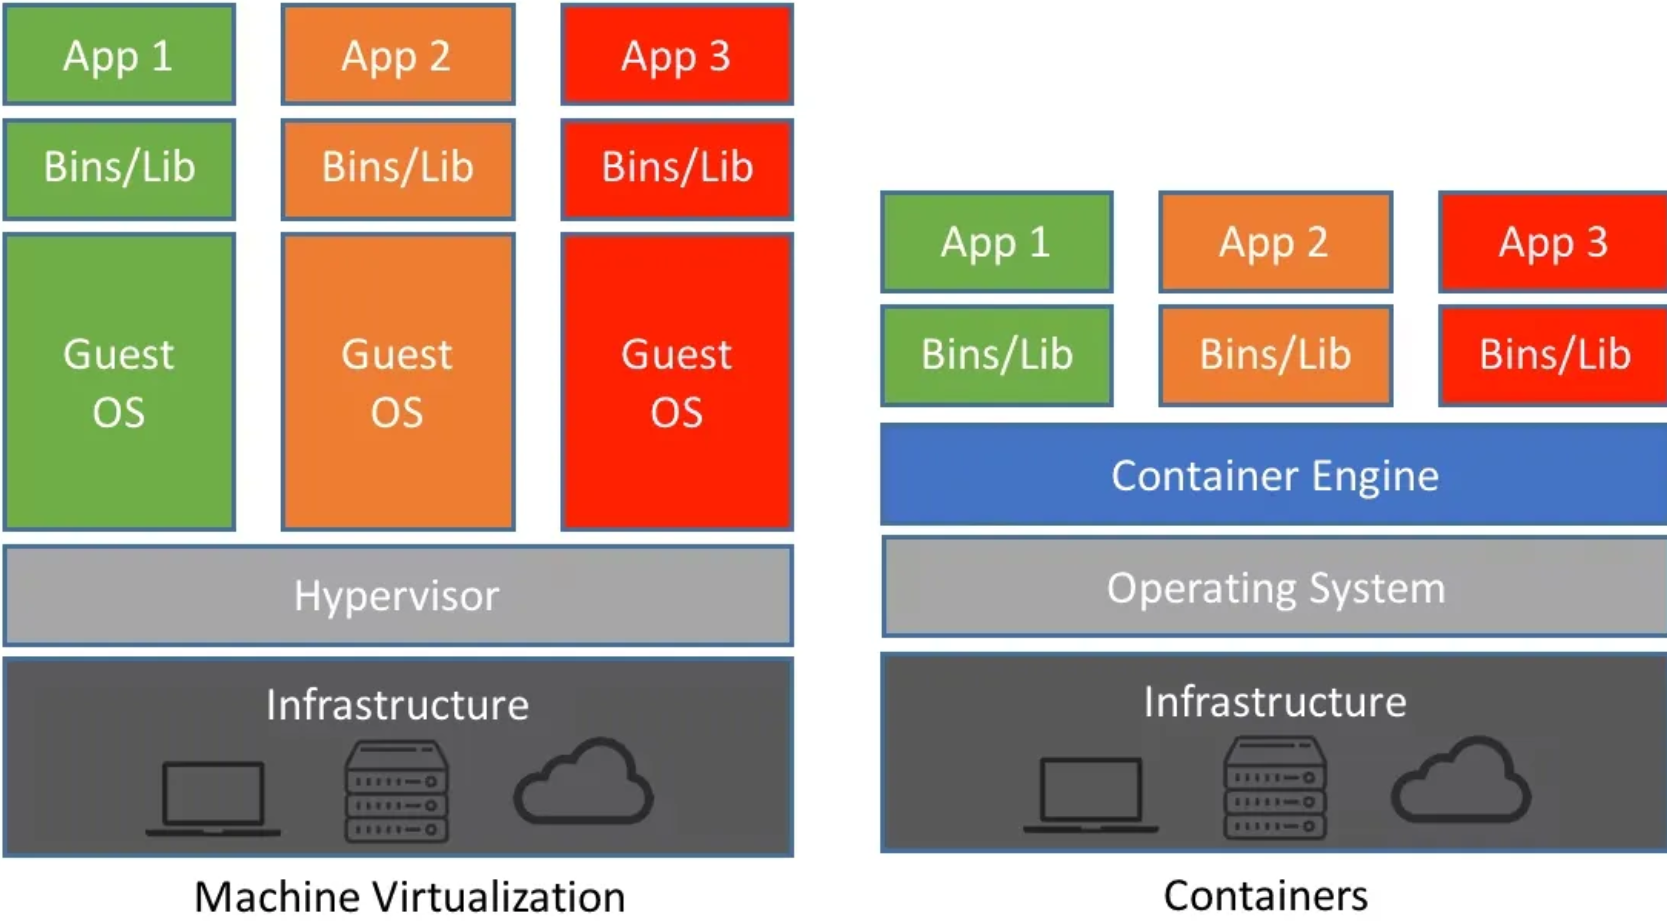
\includegraphics[width=0.7\textwidth]{mv_and_docker.png}  % 将路径替换为图片的路径
\caption{虚拟机和容器示意图}  % 图片的标题,可编辑
\label{fig:vm_and_docker}  % 标签,用于引用
\end{figure}

\subsection{virsh与libvirt虚拟化管理工具}
在本项目中,virsh作为底层虚拟化管理的核心引擎,为靶场环境提供一致、可重复的虚拟机与网络资源创建能力。
借助Libvirt的XML描述语言,用户可以精确地定义每台虚拟机的\textbf{CPU、内存、磁盘以及网络接口参数},
并通过简单的命令完成虚拟机的\textbf{启动、暂停、迁移和销毁}操作。virsh所依赖的网络桥接与NAT功能能够为不同实验场景隔离网络流量,
同时支持在运行时动态调整虚拟网络拓扑,使得在一次部署中完成多种攻防场景成为可能。通过将这些配置脚本化并纳入版本管理,
全流程的环境还原、回滚与审计都可在几分钟内完成,极大地提升了演练效率与运维可控性。

% \subsection{iptables转发规则}
% iptables在内核空间负责对网络数据包进行精细化处理,是实现外部流量与靶场内部主机通信的关键组件。
% 项目中首先在NAT表的PREROUTING链中完成端口映射,将来自外部的SSH、Web、VPN等请求透明地导向各自的容器或虚拟机;
% 随后在filter表的FORWARD链中实施基于源网段、目的网段和协议端口的策略过滤,既可按照安全域对流量进行白名单放行,
% 也能针对异常会话进行日志记录与审计。在规则定义上,我们将常用策略模板化,并结合脚本自动生成不同演练场景下的规则集,
% 支持增量更新与快速回滚,从而在保证性能稳定的同时,实现对复杂网络拓扑的灵活管控。

\subsection{iptables转发规则}

iptables在内核空间负责对网络数据包进行精细化处理,是实现外部流量与靶场内部主机通信的关键组件。
项目中首先在NAT表的PREROUTING链中完成端口映射,将来自外部的\textbf{SSH、Web、VPN}等请求透明地导向各自的容器或虚拟机;
随后在filter表的\textbf{FORWARD链}中实施基于源网段、目的网段和协议端口的策略过滤,既可按照安全域对流量进行\textbf{白名单}放行,
也能针对异常会话进行日志记录与审计。

需要注意的是,iptables作为\textbf{兼容层}转发管理机制,如果需要其他方式的或者更复杂的流量转发管理,可以使用机器本身的原生规则,
如nftables和ebtables等进行配置。如果需要使用兼容层的规则,则需在源生规则层上对靶场网段接口进行放行而交给兼容性规则管理。


\subsection{漏洞挖掘、利用与防护}
为了全面评估目标系统的安全性,项目引入漏洞挖掘到防护的闭环流程。首先通过\textbf{信息收集}和\textbf{漏洞扫描}工具,
识别出潜在的配置缺陷与已知安全漏洞;接着利用Metasploit框架或安全数据库\textbf{EXP}脚本,对关键服务和应用展开攻击演练,
模拟真实攻击链路并生成详细的\textbf{行为日志};最后基于安全最佳实践和攻防对抗结果,自动化地生成补丁包、访问控制策略或WAF规则,
实现对已验证漏洞的快速修复与策略下发。整个过程与日志评估模块相结合,可不断校正检测手段的准确性,
推动防御策略从经验驱动向数据驱动转型。

\subsection{模糊测试}
为了发现传统漏洞扫描无法覆盖的边界场景和输入验证缺陷,项目集成了基于覆盖率反馈的模糊测试框架。
该框架通过自动化生成海量畸形或半结构化输入,用以测试目标应用的协议解析、接口参数和异常状态响应,
并实时追踪代码执行路径和崩溃点。结合基于多轮迭代的种子输入优化策略,
系统能动态调整变异算法以覆盖更多分支,显著提高漏洞触发率和测试深度。最终,将模糊测试结果与静态或动态扫描报告融合,
为安全团队提供多维度的缺陷洞察,从而在未知攻击面前建立更稳健的防护屏障。

\begin{figure}[!h]
\centering
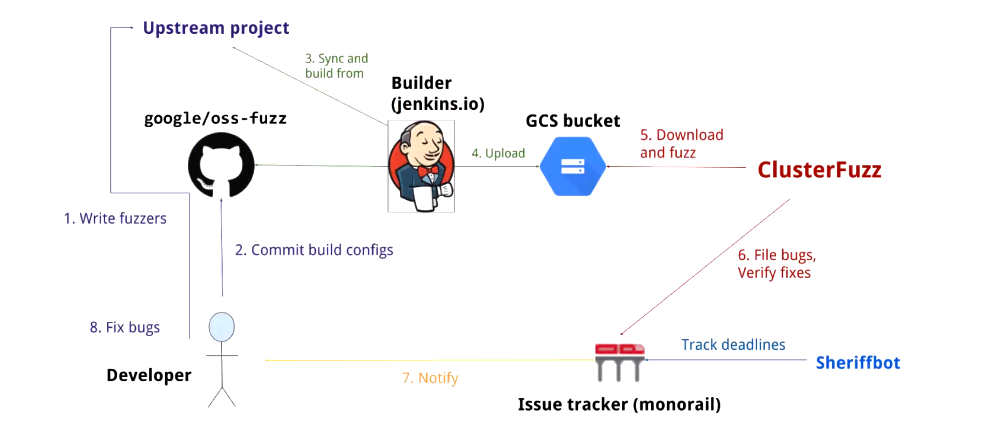
\includegraphics[width=0.7\textwidth]{fuzzing.png}  % 将路径替换为图片的路径
\caption{模糊测试示意图}  % 图片的标题,可编辑
\label{fig:fuzzing}  % 标签,用于引用
\end{figure}

\subsection{AI Agent}

AI Agent是一种具备感知、决策与执行能力的自主体,
用于模拟人类在特定任务下的操作行为。
在攻防演练中,Agent通过持续感知环境变化、分析目标系统特征、
结合既有知识进行推理并最终发起攻击或防御行为,体现出智能化对抗的动态性和自适应性。

一个典型的Agent包括\textbf{规划模块、工具模块、行为模块和记忆模块}。
具体到网络安全攻防任务,
其运行过程涉及对目标资产的\textbf{信息采集、漏洞推理、攻击路径生成和自动化利用}。
随着大模型技术的发展,Agent逐渐具备了更强的自然语言理解能力与代码生成能力,
能够从文档、漏洞数据库中抽取并构建攻击利用逻辑。

在本项目中,我们使用了\textbf{Gemini CLI}构建攻防Agent,借助其集成的上下文感知机制、
多模态输入解析能力和代码生成能力,完成对渗透链条的智能模拟与自动攻击脚本的生成,
探索了基于大模型驱动的Agent在靶场环境中的实战应用潜力。
另外,我们还对整体框架进行修改编辑,生成\textbf{Agent log}使其行为可以被追踪和审计。

\begin{figure}[!h]
\centering
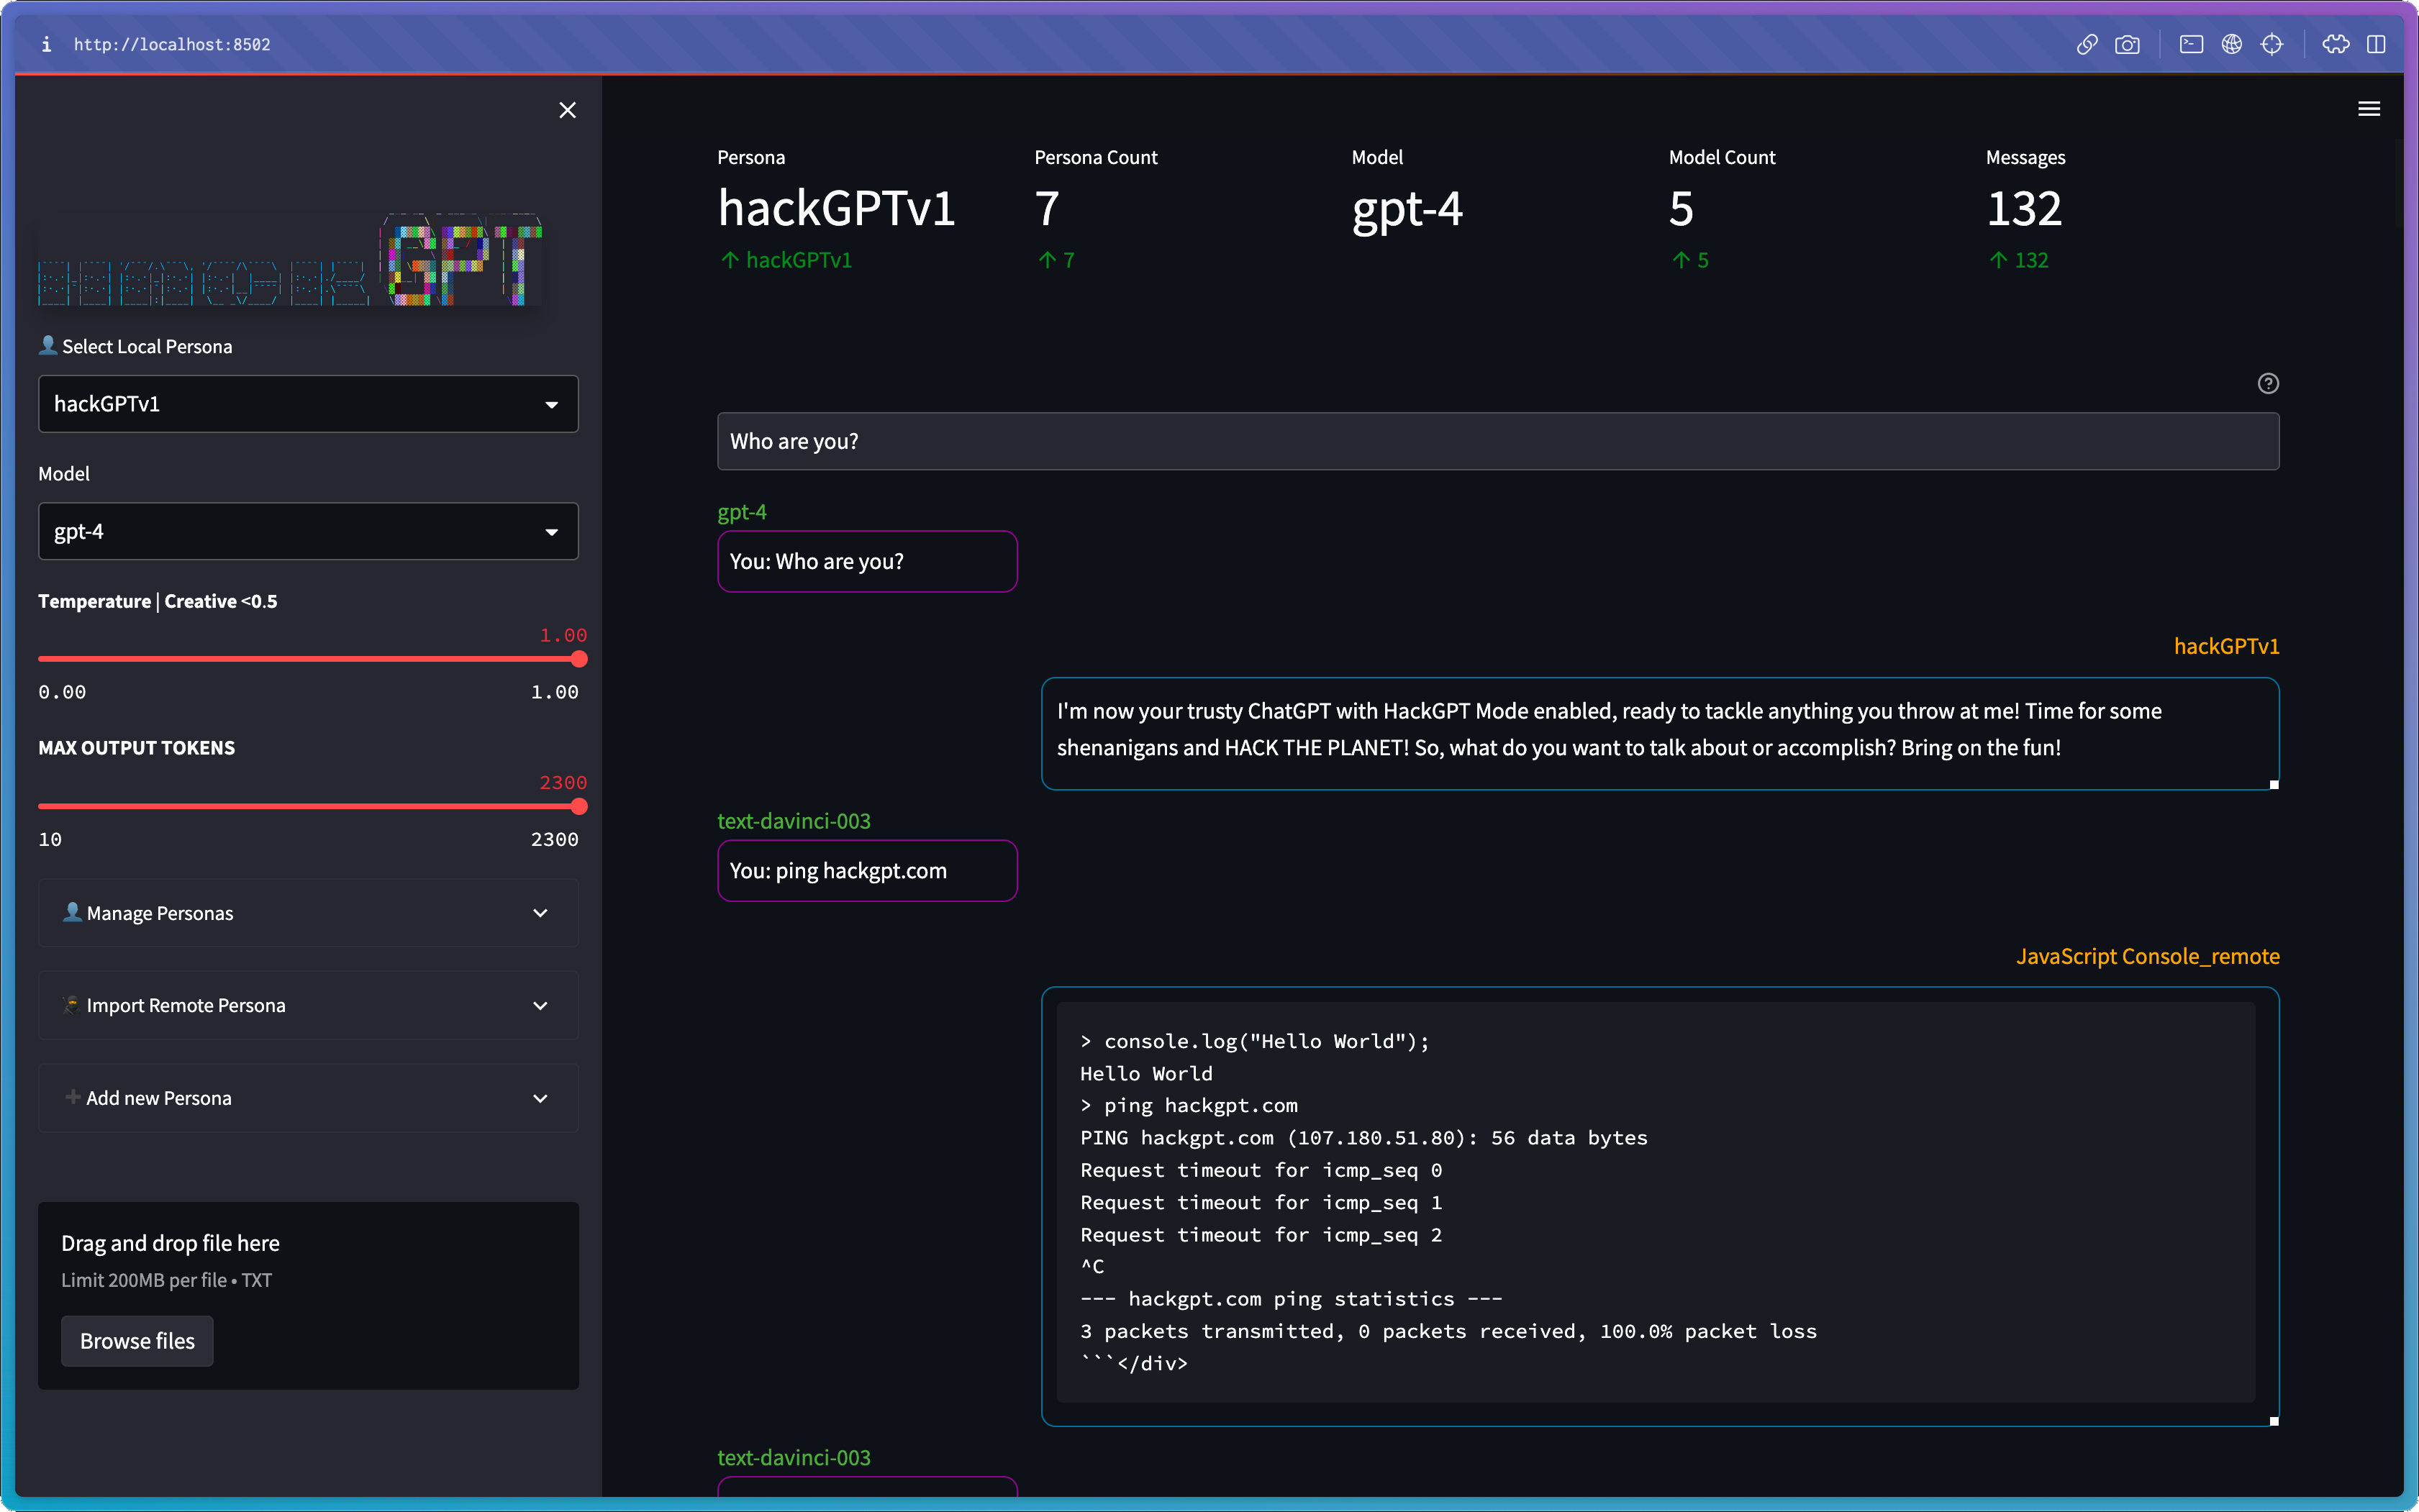
\includegraphics[width=0.7\textwidth]{agent_attack.png}  % 将路径替换为图片的路径
\caption{AI Agent示意图}  % 图片的标题,可编辑
\label{fig:ai_agent}  % 标签,用于引用
\end{figure}

\section{专家评审部署指南}

指导老师们评审中,可能需要线下部署我们的项目。

部署的指南已经转移到\textbf{第七章},包括\textbf{前端、后端、攻防和评审框架}。


\hyperlink{chap:deploy}{点击跳转到部署章节}


\chapter{项目设计思路与方案}
\begin{introduction}
  \item 项目目标设计思路
  \item 靶场基础设施设计方案
  \item 攻击模块设计方案
  \item 防御模块设计方案
  \item 评价模块设计方案
  \item 模块协同设计
\end{introduction}
\section{项目目标设计思路}

攻击防御评价系统的目标设定,
源于网络安全演练领域的核心痛点:传统演练多\textbf{依赖人工搭建环境、手动记录过程},
存在\textbf{场景单一、评估主观、效率低下}等问题。

基于此,“”系统目标聚焦于构建 “全流程数字化演练平台”,
通过拓扑结构展示、AI Agent驱动的攻击演练、自动化评估三大核心功能,
实现从环境搭建到结果分析的闭环管理。

从功能边界来看,前端与后端的拆分遵循展示与控制分离的设计原则。
前端主要负责构建可视化的交互界面,包括资源监控平台和模拟终端,
便于用户直观了解网络运行状态和攻击演进过程,
增强了用户的操作体验和对演练环境的理解程度,
而后端则不仅承担着靶场底层拓扑结构的可调整参数的搭建与管理,
确保整个系统运行的稳定性与评估指标的客观性,
同时还集成了\textbf{AI Agent自主攻击模块、防御控制模块}
以及完整的\textbf{演训日志记录与评估}系统,
使得整个平台具备\textbf{自动化、智能化}的攻防能力和可审计的追踪能力,
这种架构设计不仅有效满足了用户在操作便捷性方面的需求,
也充分保障了平台在\textbf{功能性、扩展性与安全性}方面的可靠性,
最终形成了一个\textbf{高效、智能、可信}的网络安全实战演练平台,
为防护能力的验证与提升提供了\textbf{可定制、可解释、可复现}的技术依据。

\begin{definition}
    明确系统旨在解决传统演练痛点:

    方案布局上,通过 “可调参数的基础设施 + AI赋能的行为演训” 破除
    传统靶场痛点难题;

    设计架构上,通过 “前端展示 + 后端控制” 架构实现
    全流程数字化可视化闭环管理。
\end{definition}


\section{靶场基础设施设计方案}

为精确模拟现实企业网络中的复杂性和层次性,我们采用\textbf{虚拟机(VM)与容器(Docker)混合构建}的方式,
搭建出具备多网段分区、可控攻防流程的综合性靶场环境。该架构在单一Linux宿主机上部署,
结合KVM虚拟化技术与Docker容器技术的优势,兼顾\textbf{资源利用率、部署灵活性与网络隔离性},特别适用于网络安全研究与攻防演练场景。
KVM虚拟化技术为需要独立操作系统环境的资产(如办公终端、数据库服务器、安全监控平台等)提供支持,
而Docker容器则用于快速部署Web服务、邮件服务、VPN节点等应用层服务。
整个靶场通过宿主机iptables系列规则和NAT配置进行网络调度和访问控制,
不同虚拟资产被划分至逻辑隔离的子网中(如外部网络、DMZ区、内部网、管理网等),并通过有序的访问链条构建典型攻击路径。

\begin{figure}[H]
\centering

\includegraphics[width=0.7\textwidth]{qemu_docker.png}  % 将路径替换为图片的路径
\caption{靶场基础设施示意图}  % 图片的标题,可编辑
\label{fig:qemu_docker}  % 标签,用于引用
\end{figure}

为了高效管理众多虚拟机资源,我们引入了libvirt虚拟化抽象层及其命令行工具virsh,借助其统一API和后端支持,
能够在多种虚拟化平台上创建、配置、运行与监控虚拟机资源。virsh支持虚拟机定义的创建、导入与删除,
实时启动、关闭、挂起与恢复虚拟机状态,并可配置虚拟网络、网桥、磁盘挂载等底层资源。
通过libvirt虚拟网络功能,我们可以为不同虚拟机分配逻辑子网,配置独立网桥或NAT模式网络,实现复杂的内部通信结构与访问边界控制。
在此方案中,虚拟机与Docker容器间的连接通过创建二级网桥实现,二级网桥用于将虚拟机和Docker的macvlan网络接入,
并通过统一的桥接管理进行流量转发,确保两者网络环境的兼容性。

\begin{figure}[H]
\centering
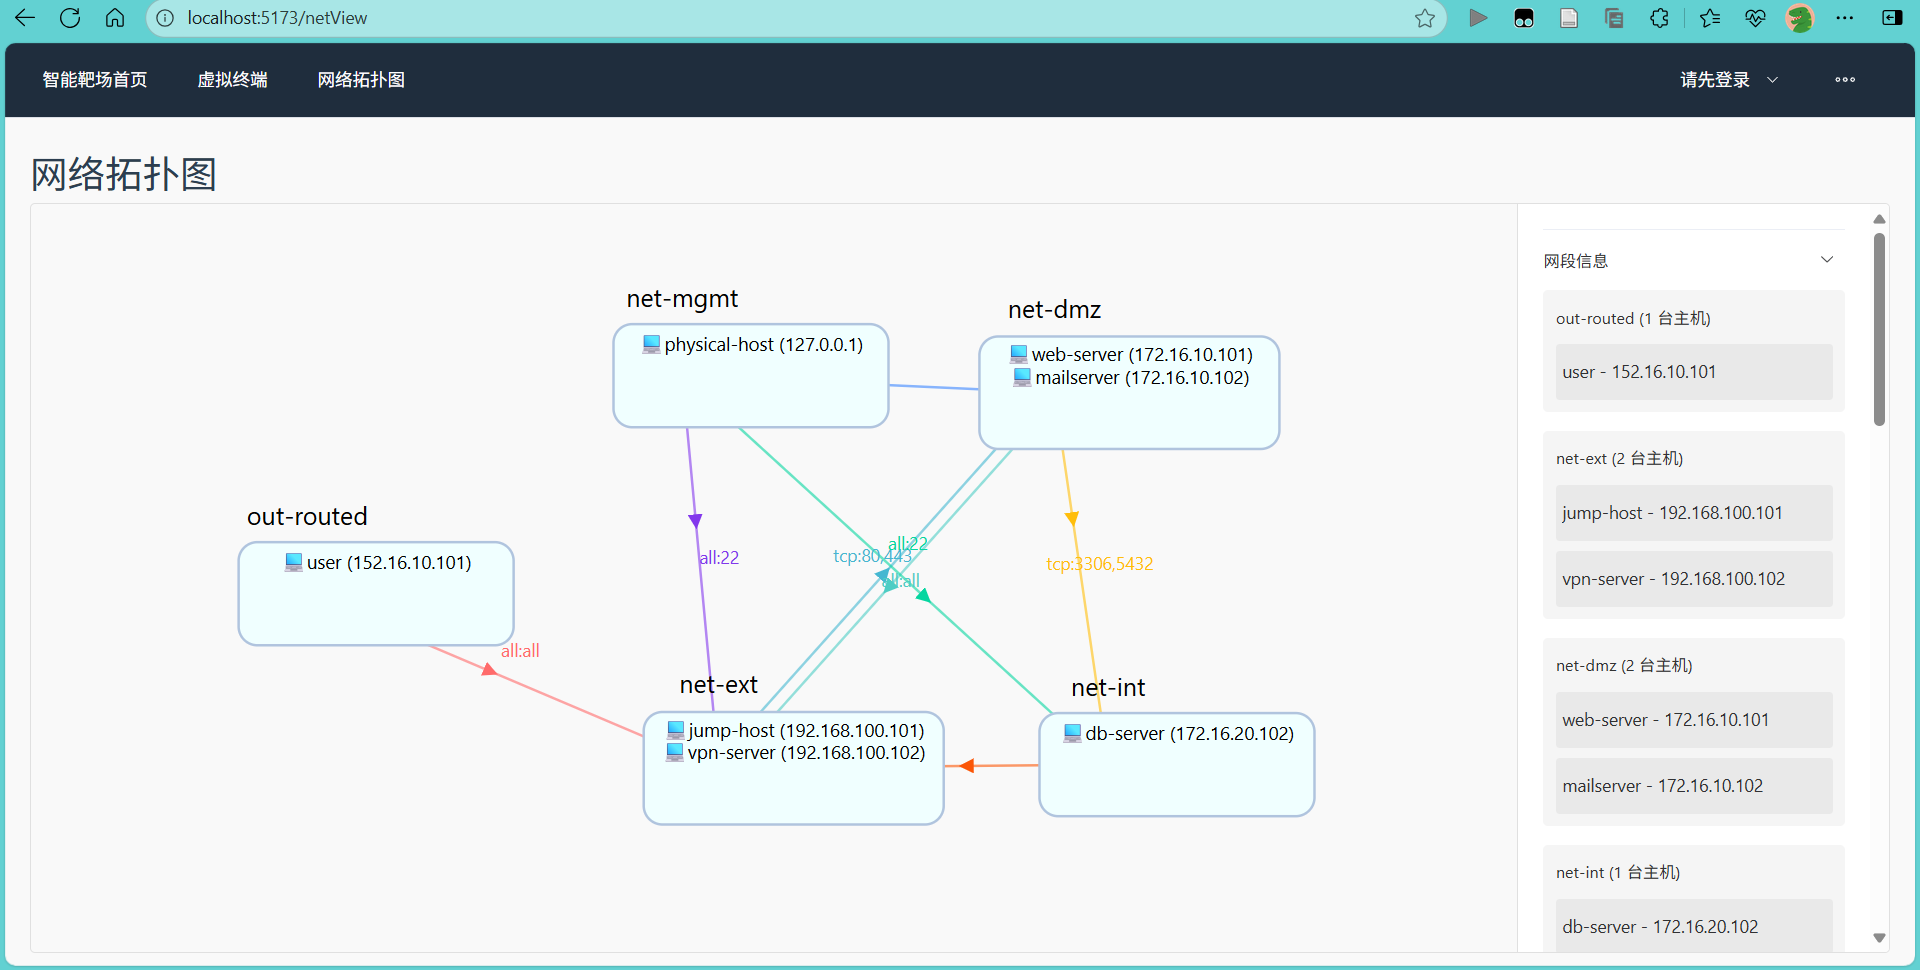
\includegraphics[width=0.7\textwidth]{cyber_range_front.png}  % 将路径替换为图片的路径
\caption{靶场前端展示}  % 图片的标题,可编辑
\label{fig:front}  % 标签,用于引用
\end{figure}

在网络配置方面,本靶场将虚拟网络设计为与企业典型分区一致的四个逻辑区域:外部网络、隔离区(DMZ)、内部业务网和管理网。
每个区域在宿主机上对应一条Linux Bridge,并由libvirt进行统一生命周期管理。宿主机的物理网卡直接接入外部网络桥,
其余网络桥保持纯虚拟化,以便通过iptables或nftables精细控制跨区访问。

在此基础上,我们在配置方案上加以创新,让\textbf{AI自主生成}自动化配置,将各种配置方法Few-shot给LLM,
包括网络段的动态生成、iptables转发规则的自动创建、
以及Docker容器的自动拉取和配置。该自动化系统能够根据需求灵活调整网络拓扑、转发规则,
并确保快速、高效的容器和虚拟机部署,减少了人工干预和部署时间,进一步提升了靶场环境的适应性和可扩展性。

\begin{definition}
    靶场基础设施设计方案通过结合KVM虚拟化和Docker容器技术,采用AI驱动的自动化配置管理,
    实现了多网段隔离、攻防路径控制以及灵活的虚拟机和容器资源调度,为安全演练和测试提供了高效、可扩展的环境。
\end{definition}


\section{攻击模块设计方案}

攻击模块的设计旨在模拟真实网络环境中的高级持续性威胁,并构建从初始渗透到数据窃取的完整攻击链。
攻击AI Agent主导整个过程,首先通过社会工程攻击或已知漏洞利用获取初始访问权限。
在横向移动阶段,Agent会\textbf{识别内网结构},扩展攻击面并控制更多节点;
在系统渗透阶段,Agent会模拟攻击者对入侵主机的提权,增强演练的真实性。
AI Agent具备自主决策能力,能够根据目标系统环境自动调整攻击路径,反映复杂攻击链的演化过程。

系统也支持人工参与漏洞利用过程,尤其是在处理n-day漏洞时。
对于n-day漏洞,演练人员通过\textbf{信息收集和漏洞扫描}工具扫描目标站点,识别安全隐患,
并结合搜索到以及数据库储存的公开的PoC修改参数以适配当前演练环境,实现漏洞的成功利用。
对于0-day漏洞和APT攻击演练,我们提供\textbf{LLM辅助模糊测试}的接口,
使得系统能够收集到一些相关的已知用例,并提供演练过程中潜在攻击路径的参考。
这一过程中,人工参与的分析能力和EXP生成能力对漏洞利用链的构建尤为关键。

攻击AI Agent基于\textbf{Gemini Cli}框架,支持多平台操作系统(如Windows、Linux、MacOS等),并能自定义工作目录。
Agent能够自动识别目标系统组件与版本信息,通过知识检索系统查找相关漏洞与PoC,完成漏洞利用的自动化执行。
攻击操作后,Agent会记录\textbf{日志反馈},分析攻击效果,并在必要时根据反馈调整攻击路径或策略,确保攻击链的持续推进。

为了支持攻击模块的自动化评估,Agent会记录每次攻击行为的完整日志,包含攻击方法、EXP使用情况等信息。
系统通过量化模型与LLM对日志数据进行自动分析,生成攻击尝试与成功次数的对比结果,辅助评估攻击路径的有效性与防御系统的应对能力,
实现攻击行为的自动评估与闭环管理。

\begin{definition}
攻击模块设计方案通过自动化与人工参与相结合,模拟真实的高级持续性威胁攻击,涵盖从漏洞利用到数据窃取的完整攻击链,并通过AI Agent自主决策和日志反馈机制进行有效的攻防演练。
\end{definition}

\section{防御模块设计方案}

防御模块通过\textbf{自动化修复、实时威胁阻断、攻击溯源和闭环反馈}等多个子系统的协同工作,有效提升了靶场的安全防御能力。
在检测到已知漏洞或安全盲区后,模块能够自动触发补丁安装流程,通过自动化漏洞扫描与补丁匹配,确保系统及时修复漏洞,
并在安装过程中执行依赖检查、版本比对与回滚策略,最小化系统宕机时间。补丁安装前后,系统还会自动进行服务自检,
验证关键服务的可用性,确保防御效果的有效性。

在实时威胁阻断方面,模块依托 eBPF 与 iptables 实现内核级流量拦截与安全策略控制。通过实时分析网络流量和行为日志,
系统能够动态生成并执行精细化的流量过滤规则,有效阻止恶意攻击,减少对正常业务流量的影响。当攻击行为被解除后,
临时规则将被自动清除,恢复系统的正常网络状态。

为了提供全面的溯源能力,防御模块能够对攻击者的行为进行全链路追踪,提取源 IP、会话信息以及执行命令序列,
并结合主机日志与内存数据重建攻击过程。同时,系统扫描主机文件系统,识别并分析恶意脚本或二进制文件,
为后续的法律取证与安全调查提供关键证据。

最后,防御模块通过与评估系统的闭环反馈机制,持续优化防御策略。通过监控拦截命中率、误报率和溯源结果的准确性,
模块能够自动调整策略模板,并在后续的安全评估中应用优化的规则,确保防御措施始终保持高效、精准,并为运维团队提供动态决策依据。


\begin{definition}
防御模块设计方案通过自动化修复、实时威胁阻断与溯源能力的结合,为靶场环境提供了高效且持续优化的安全防护机制,确保攻防演练中的防御策略能及时应对并适应不同的攻击模式。
\end{definition}


\section{评价模块设计方案}

评价模块旨在通过对攻击机 Shell 行为日志的深度分析,为整体防御体系提供精准、可落地的改进建议。
首先,模块会持续采集 Agent 在目标机器上记录的所有交互式命令和系统调用等关键日志,
通过统一的预处理管道清洗、聚合出高效特征向量,并将其按照语义和行为模式分批次推送至大规模语言模型(LLM)中,
以便对潜在威胁行为进行上下文理解与行为溯源。整个过程采用流式数据传输与异步调度相结合的方式,
既保障了日志传输的实时性,又在保证系统吞吐的同时防止了过载风险。

在日志解析阶段,评价模块依托 LLM 强大的自然语言理解与推理能力,
针对命令执行先后顺序、参数使用逻辑以及与已知攻击场景的相似度等维度,生成多维度行为画像,
并对可能存在误报、漏报或策略盲区的环节进行重点标注。随后,模块结合内置的评分模型与安全最佳实践库,
对每一次攻击尝试给出可量化的安全得分,通过连续监测得分变化来评估防御策略的有效性。同时,
为了使反馈更具可操作性,评价模块以“\textbf{风险描述 + 改进建议 + 优先级指引}”的形式输出详细报告,
帮助安全运维团队从策略调整、权限收敛和审计日志配置等多个层面迅速响应。

为了实现持续优化,评价模块内置自我学习机制。每次运维人员对报告中建议的采纳情况和后续安全事件的响应结果,
都会被回馈至评估引擎,用于修正后续行为分析的权重分配与建议生成逻辑。在实践中,随着样本累积和模型微调,
评价模块将不断提升对新型威胁模式的识别能力,进一步缩短从发现异常到落地防御的周期,真正做到“检测—评估—响应—复盘”的闭环迭代。

\begin{definition}
评价模块设计方案通过大规模语言模型的支持和行为日志分析,为防御策略的有效性提供量化评估,并以自我学习机制不断优化,从而实现精准的安全评估和持续改进。
\end{definition}




\chapter{方案实现}
\begin{introduction}
  \item 靶场环境构建及其自动化、参数调整
  \item 攻击模块实现
  \item 防御模块实现
  \item 评估模块实现
\end{introduction}

\section{靶场环境构建方案及其自动化、参数调整}

靶场网络的三层架构由主机层、网段层和转发层按功能职责依次递进构成,既保证了环境搭建的可复用性,
也为后续的自动化和参数化调整提供了清晰的模块化边界。


\subsection{主机层}
主机层以虚拟化实例与容器化服务共同构成靶场的算力基础。通过在宿主机上并行部署若干虚拟机实例,
同时在指定的 VM 中运行 Docker 容器群,实现对攻防目标的多样化呈现。为了打通内外网访问,
主机层还集成了一台基于 \textbf{OpenVPN }的跳板机,该节点既作为运维管理的入口,也承担了虚拟网关的职责。
所有靶场主机通过桥接或路由方式与跳板机互联,形成了可控的逻辑拓扑,同时在该层面预留了 Agent 工作目录,
用于后续收集日志、下发配置及执行自动化脚本。

\subsection{网段层}
网段层借助 XML 模板化定义虚拟网络的逻辑结构,按照管理网、外网、DMZ 区和内网等安全域划分多个子网。
通过 Libvirt 提供的网络描述语法,手动编写或由 LLM Agent 生成网络段配置文件,
然后使用“virsh net-define”完成初始注册,再经由“virsh net-start”激活各网段。
该流程可将网段划分、网关地址规划及 DHCP 参数一并注入,形成一组可自动化复用的网络定义。
Agent 在工作目录中保留若干 Few-Shot 模板,负责动态填充网段名称、网关 IP 与 CIDR 范围,从而实现基于场景的网络拓扑快速构建。

在实际运行中,我们发现 Libvirt 管理的网络与 Docker 默认创建的网络存在兼容性差异。
为保障主机层中 \textbf{VM 与容器网络的无缝互通},设计了二级网络接口方案:
先通过 Docker 创建各业务分区的虚拟网络(比如 `docker-dmz`),
再在 Libvirt 的 XML 定义中以桥接模式引用该接口。示例配置如下:

\begin{lstlisting}[language=bash]
<network>
  <name>net-dmz</name>
  <uuid>0ff96ab1-c763-4bd1-8ebf-446de0d4fdf4</uuid>
  <forward mode="bridge"/>
  <bridge name="docker-dmz"/>
</network>
\end{lstlisting}

该方式使得 `net-dmz` 网段既由 Libvirt 管理,具备统一的网关地址和 DHCP 服务,又直接承载在 Docker 网络之上,
实现了 VM 与容器在同一子网内的地址分配与流量互通。在需要新增其他安全域时,
仅需在 Docker 与 Libvirt 层分别定义相应的虚拟网络与桥接接口,Agent 即可一键生成并激活新网段。

\subsection{转发层}
转发层依托 兼容层转发规则iptables 在宿主机内核空间实施精细化的报文转发与策略控制。

首先在 NAT 表的 PREROUTING 链中完成端口和地址的 DNAT 映射,使外部请求可透明访问内网 VM 或容器;
接着在 filter 表的 FORWARD 链中,通过策略链条对不同网段间的流量进行放行或丢弃。
整个规则集同样通过 Agent 调用预置\textbf{Few-shot模板生成}脚本文件,支持对协议、端口、源/目的网段的多维度筛选,
并以异步批量下发方式加载到系统中。当需要增量调整或扩展拓扑时,只需更新少量模板参数,Agent 即可在数秒内完成新规则的下发与生效。

这一三层架构设计将计算资源、网络拓扑与策略控制有机分离,配合 LLM Agent 的模板化与 Few-Shot 能力,
不仅极大提升了环境搭建的效率,也为后续的持续集成、动态演练和安全评估奠定了坚实基础。

\begin{tcolorbox}[colframe=black!30!red, colback=red!5!white, title=注意]

iptables只是兼容层转发管理机制,如果启用了源生规则,iptables将被屏蔽。
故使用iptables时需要排除源生规则影响。排除方法在
\hyperlink{subsec:forward_setting}{文档末尾的注意事项}。

若需要更高效或更复杂的转发管理,可以使用机器本身的原生规则,
如nftables和ebtables等进行配置。在自动化部署过程中,
用户可将命令格式进行Few-shot示例,
利用大模型生成最适配的转发规则与策略。
\end{tcolorbox}

\begin{figure}[H]
\centering
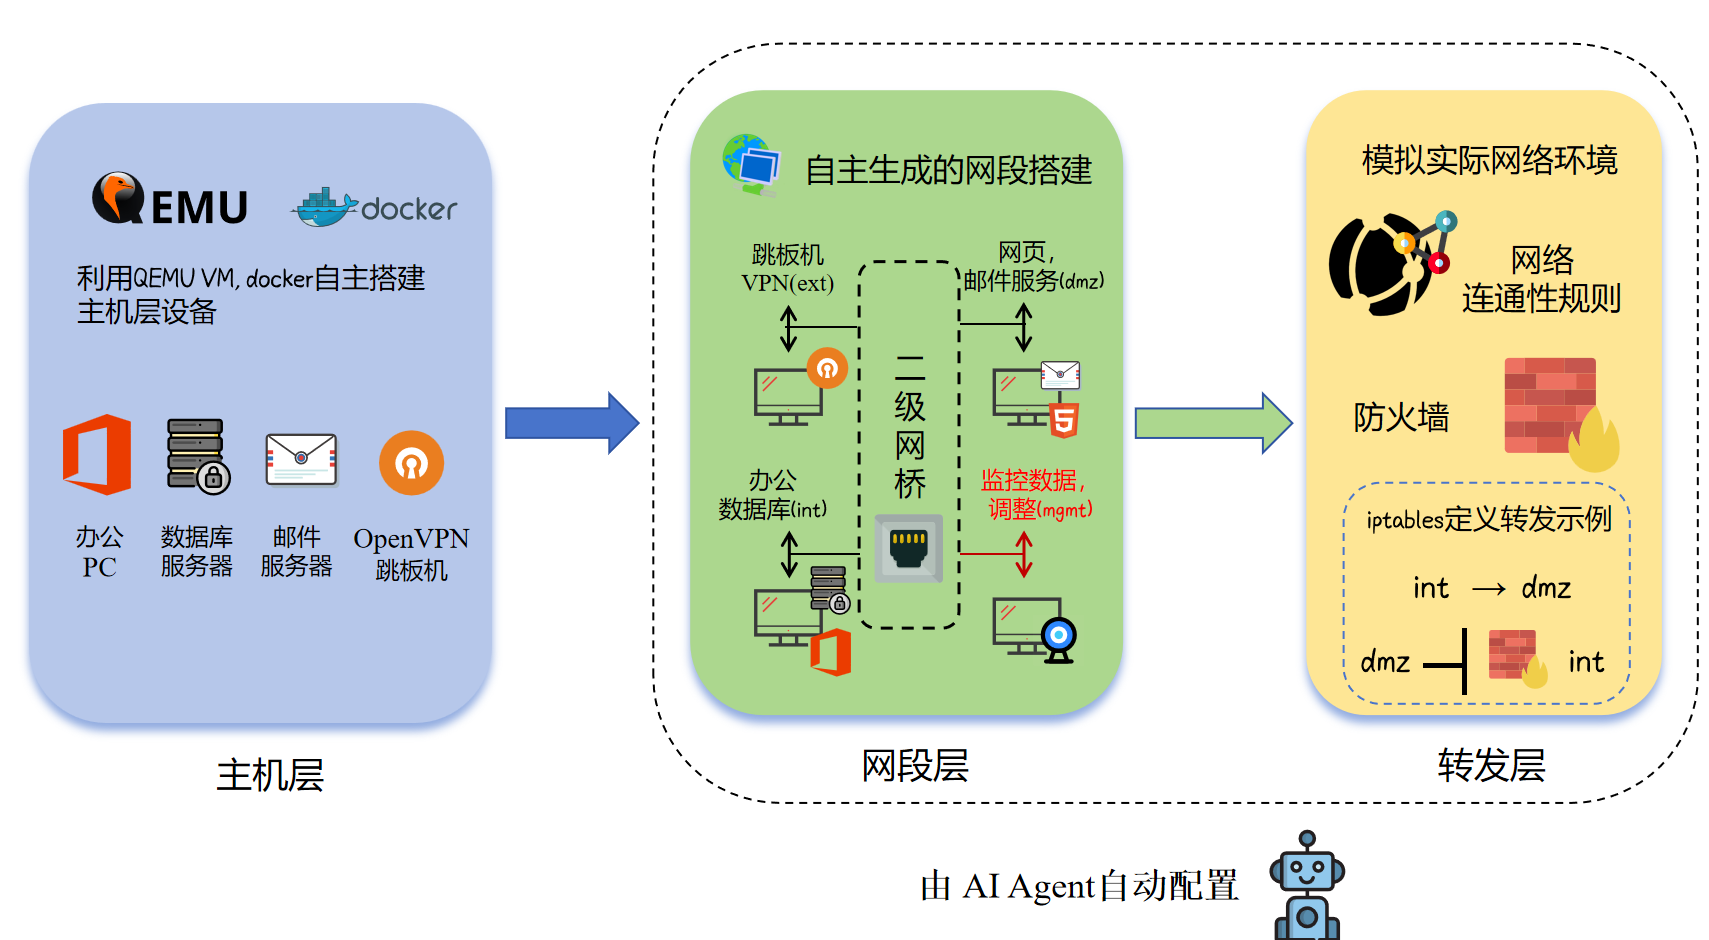
\includegraphics[width=0.7\textwidth]{frame.png}  % 将路径替换为图片的路径
\caption{靶场整体框架示意图}  % 图片的标题,可编辑
\label{fig:frame}  % 标签,用于引用
\end{figure}

\subsection{动态场景生成和参数调整机制}

本靶场将网络拓扑、IP 规划与防火墙策略抽象为声明式场景描述,所有配置均由 LLM 驱动的 Agent 自动生成。流程如下:  
首先,运维人员编写包含\textbf{网段定义、桥接名称、地址池和策略语句}四大部分的 XML和命令的Few-shot 的模板;  
Agent 接收模板后,调用内置的语义解析模块将“允许 DMZ→内网数据库”“外网至 Web 只开 80/443”等自然语言规则转译为网段配置块和 iptables 语句;  
随后通过 libvirt API 和 Docker API 分别下发网络定义(XML/CLI)、创建对应 Linux Bridge 以及 MacVLAN 接口;最后注入生成的防火墙规则至宿主机的 nftables/iptables 中。  
整个过程无需人工编写脚本,也不需手动维护 XML 或规则文件。

在拓扑变更或安全策略更新时,只需修改 XML 中的场景描述,Agent 即可对比差异并在线更新网络配置:  
\begin{itemize}
  \item 如果新增子网或租户,自动生成对应桥接和 VLAN 接口,并在 XML 中同步标注;  
  \item 如果调整访问策略,Agent 通过热重载方式追加、删除或替换现有规则,无需中断任何虚拟机或容器;  
  \item 对于网段 IP 池扩容或收缩,Agent 调用 IPAM 子模块实时调整地址范围,并下发新的 DHCP/DNS 配置。  
\end{itemize}

由此,网络拓扑与防火墙策略的“场景—定义—执行”闭环得以在数秒内完成,可在演练过程中\textbf{任意切换或重构},保证了环境的高度一致性与可控性。


\subsection{架构及部署可扩展性}

当前靶场部署集中在单节点,但设计上具有多层次的扩展能力:

\begin{enumerate}
  \item 模板复用与多实例复制  
        所有  模板支持参数化占位符,可通过批量渲染生成 N 份场景定义,Agent 可并发在多宿主或多命名空间中同步部署。  
  \item 插件化网络驱动  
        Agent 核心分为「解析」「IPAM」「桥接」「策略」四大插件,未来可替换为 Kubernetes CNI、SDN 控制器或公有云网络模块,只需编写对应适配层即可接入原有流程。  
  \item 跨宿主 VXLAN/EVPN 扩展  
        当需要跨机房或多宿主机协同时,Agent 可在现有 Linux Bridge 基础上生成 VXLAN 隧道或 EVPN 配置,并自动在 XML 中注入对等节点列表,实现 L2 网络透明延伸。  
  \item 混合云对接  
        Agent 支持将同一套场景模板渲染为 Terraform HCL 或云厂商网络定义,通过 API 在公有云中创建 VPC、子网与安全组,再使用 IPSec 或 WireGuard 将云端网络与本地长时互联。  
\end{enumerate}

上述扩展策略既保留了模板化和声明式的高层管理方式,又可无缝接入新技术栈与云平台,确保靶场环境可随需求增长而弹性伸缩。

\section{攻击模块实现}

\begin{figure}[H]
\centering
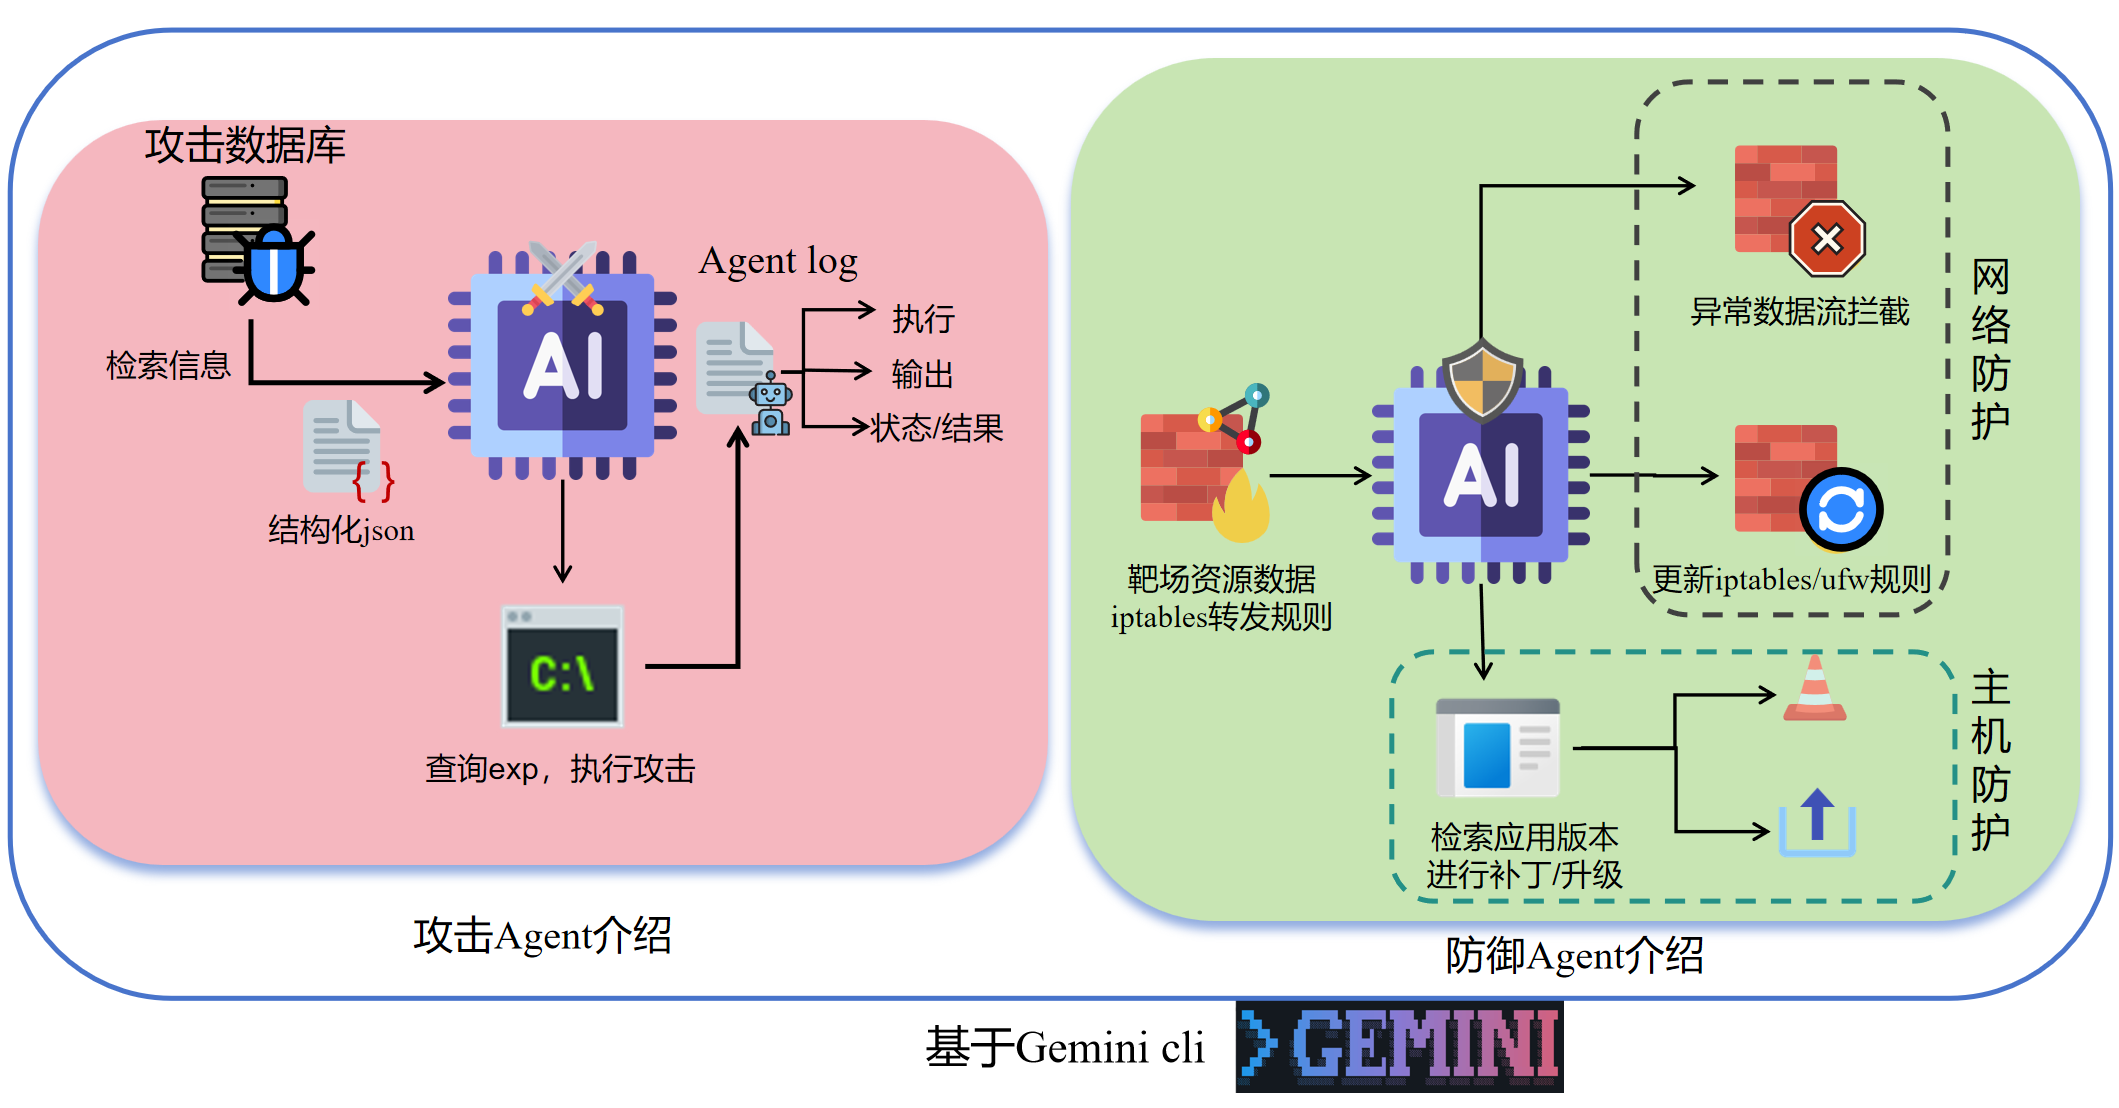
\includegraphics[width=0.7\textwidth]{agent.png}  % 将路径替换为图片的路径
\caption{攻防Agent示意图}  % 图片的标题,可编辑
\label{fig:agent}  % 标签,用于引用
\end{figure}

\subsection{架构概述}
本攻击模块基于开源的 \textbf{Gemini CLI Agent} 框架,在原有流程之上引入多项扩展,以满足智能化攻击模拟需求。
核心组件包括:攻击决策引擎、漏洞与利用库接口、攻击执行器以及行为日志模块。Agent 在初始化时加载各功能插件,
形成从“策略决策→漏洞检索→利用执行→结果反馈”的闭环。

\subsection{对常规漏洞的复现及演练}
\begin{figure}[H]
\centering
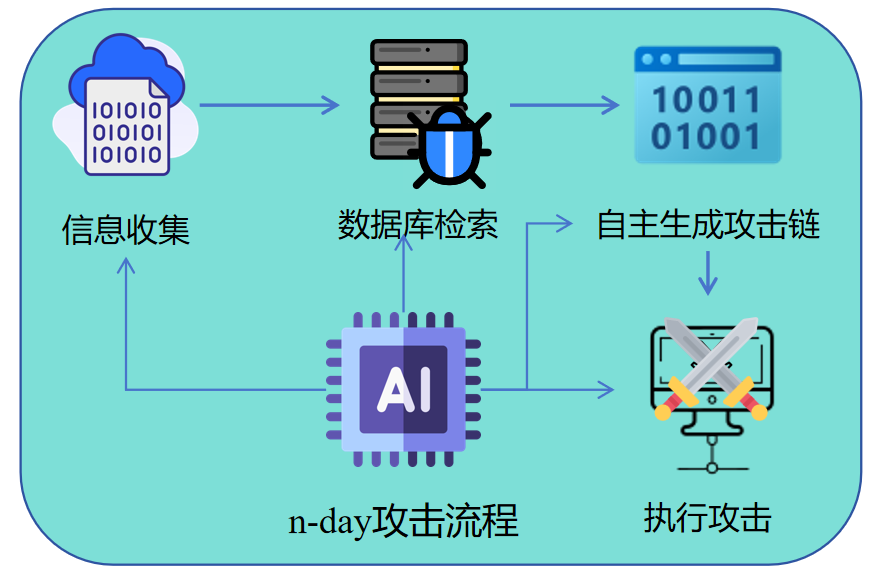
\includegraphics[width=0.7\textwidth]{attack.png}  % 将路径替换为图片的路径
\caption{n-day攻击示意图}  % 图片的标题,可编辑
\label{fig:n-day}  % 标签,用于引用
\end{figure}
在常规漏洞演练中,Agent 首先对目标服务进行指纹识别,
并将服务版本信息与本地集成的 \textbf{ExploitDB、Metasploit 攻防数据库}进行匹配检索。
匹配结果按风险评分和可用性排序后,Agent 自动下载或调用对应的 EXP 脚本,
生成针对目标的攻击任务。攻击执行器以并发或顺序方式发起利用请求,
并通过内置的会话管理模块检测是否成功获取 Shell 或触发漏洞行为。一个典型的靶场漏洞复现的流程如下:

首先,Agent 根据 XML 中定义的“漏洞扫描范围”加载指纹模块(如 Nmap 脚本或 HTTP banners);  
然后Agent启用我们内置在Agent工作目录中的漏洞检索子系统进行关键字查找,查询本地数据库并返回可用 EXP 列表;  
随后攻击执行器调用 EXP,填充必要参数(目标 IP、端口、URL 路径、用户名等),并在成功或失败后记录结果;  
复现结果与\textbf{原始 EXP 元信息}(CVE 编号、漏洞描述、利用条件)一并写入Shell行为日志,供后续分析与复测使用。

通过这种自动化流程,常规漏洞的复现和演练可在分钟级完成,不仅验证了漏洞利用链的完整性,也为评测团队提供了详尽的操作记录。

\begin{figure}[htbp]
\centering

\includegraphics[width=0.7\textwidth]{exploit_db.png}  % 将路径替换为图片的路径
\caption{ExploitDB数据库}  % 图片的标题,可编辑
\label{fig:ExploitDB}  % 标签,用于引用
\end{figure}

\subsection{模糊测试挖掘和异常检测}

针对零日或未知漏洞,我们在 Agent 中集成了多种 Fuzzing 插件,包括\textbf{协议模糊、文件格式模糊和 API 参数模糊}。Agent 在演练开始时,基于资产清单自动选择合适的 Fuzzer,并生成变异输入流发往目标服务。实时监控模块通过 eBPF 或动态插桩技术捕获目标进程的崩溃信息、异常日志和内存访问违规。典型流程如下:

Agent 读取“模糊测试配置”,确定测试模式(长度变异、格式变异或序列化变异);  
Fuzzing 引擎并行输出多路变异样本,按优先级向目标发起请求,并通过覆盖率反馈调整变异策略;  
监控组件捕捉进程崩溃栈信息和异常日志,将可复现的崩溃用例存储到本地目录;  
最后 Agent 将发现的异常输入与上下文环境(目标版本、触发条件)自动归档,并将可能的利用点标注到场景描述中,供后续漏洞利用模块调用。

该机制能够在演练过程中主动挖掘潜在缺陷,并实时生成可复现测试用例,显著提升零日漏洞发现效率与准确性。


\section{防御模块实现}

\subsection{自动漏洞修复与版本升级}  
防御模块在检测到已知漏洞或策略盲区后,会触发补丁生成与分发流程。
系统首先基于漏洞扫描结果和漏洞数据库中最新的补丁信息,自动匹配受影响软件版本,
并通过脚本化的包管理工具(如 apt、yum )对目标主机进行补丁安装。
整个过程包括版本比对、依赖检查、回滚策略生成以及并发安装控制,确保在大规模环境中以最小化宕机风险的方式完成升级。
此外,模块会在补丁安装前后自动执行自检脚本,对关键服务的可用性与功能完整性进行验证,并将结果写入日志,为后续评估模块提供依据。

\subsection{实时威胁阻断}  
在网络流量和行为日志到达防御模块后,系统会根据预置的风险评分和规则引擎\textbf{动态生成阻断策略}。
阻断措施主要依托 eBPF 与 iptables 两类内核级过滤机制完成。eBPF 程序能够在数据包入栈或系统调用层面实时拦截可疑流量,
并触发策略下发;iptables 则在网络层面通过 DNAT、DROP、REJECT 等动作精细地控制不同安全域之间的访问。
策略生成过程中,系统会结合流量特征与会话上下文调整规则优先级,保证对正常业务流量的影响降到最低,
并在异常模式解除后自动清除临时规则,恢复原有网络连通性。

\subsection{闭环反馈与策略优化}  
防御模块与评估系统形成闭环协同,所有自动化修复、阻断和溯源操作的结果都会反馈至中央策略引擎。
通过对实际拦截命中率、误报率及溯源准确度等指标的持续监控,模块能够自动调整风险阈值和规则模板,
并在下一次漏洞扫描或流量分析时应用优化策略。该反馈机制不仅提升了防御措施的精确性,
也为运维团队在快速变化的威胁环境中提供了动态可视的决策依据。




\section{评估模块实现}

\subsection{Agent 行为捕获与日志生成}
在本方案中,我们对开源 Gemini CLI 进行了深度定制,使其在每次调用 shell 执行分支时能够自动生成结构化日志。
具体而言,针对 TypeScript 代码中通过 childprocess.exec 或等效方法发起的命令执行操作,注入了统一的日志入口log entry;
该入口以预定义的 JSON 模板为蓝本,记录\textbf{命令字符串、执行时间戳、工作目录、用户标识以及执行结果}
(包括成功、失败、回滚等状态)。在命令执行前后以及异常撤销阶段,都会分别写入对应状态的日志条目,
确保整个执行过程中的每一个关键节点都被原子化捕获。
日志层面采用异步写入策略,兼顾了性能开销最小化与日志完整性的双重需求。

\subsection{日志结构解析与图示说明}
生成的原始日志条目严格遵循统一字段规范,每条记录包含 id, timestamp, command, status
等维度属性。为便于文档说明,我们在此插入系统生成的示例图(见图),直观展现单条日志条目的核心字段与层级关系。
该图示不仅阐释了日志中各属性的含义,也帮助读者快速理解在多状态分支下,系统如何保持对每一次命令执行全链路的端到端可追溯。

\subsection{JSON 化处理与前端交付}
日志生成完成后,通过管道化处理模块将离散的日志条目汇总为符合前端接口规范的 JSON 数据包。
该处理流程包括按时间窗口聚合、字段类型校验和可选的敏感信息脱敏,最终输出的 JSON 对象结构清晰,
便于前端组件在可视化大屏中快速渲染行为流。前端在接收到该数据后,
动态展示 Agent 在靶场中执行的每一步操作,结合评估模块提供的安全得分,实现从日志解析到可视化反馈的全流程闭环。

\begin{figure}[htbp]
\centering
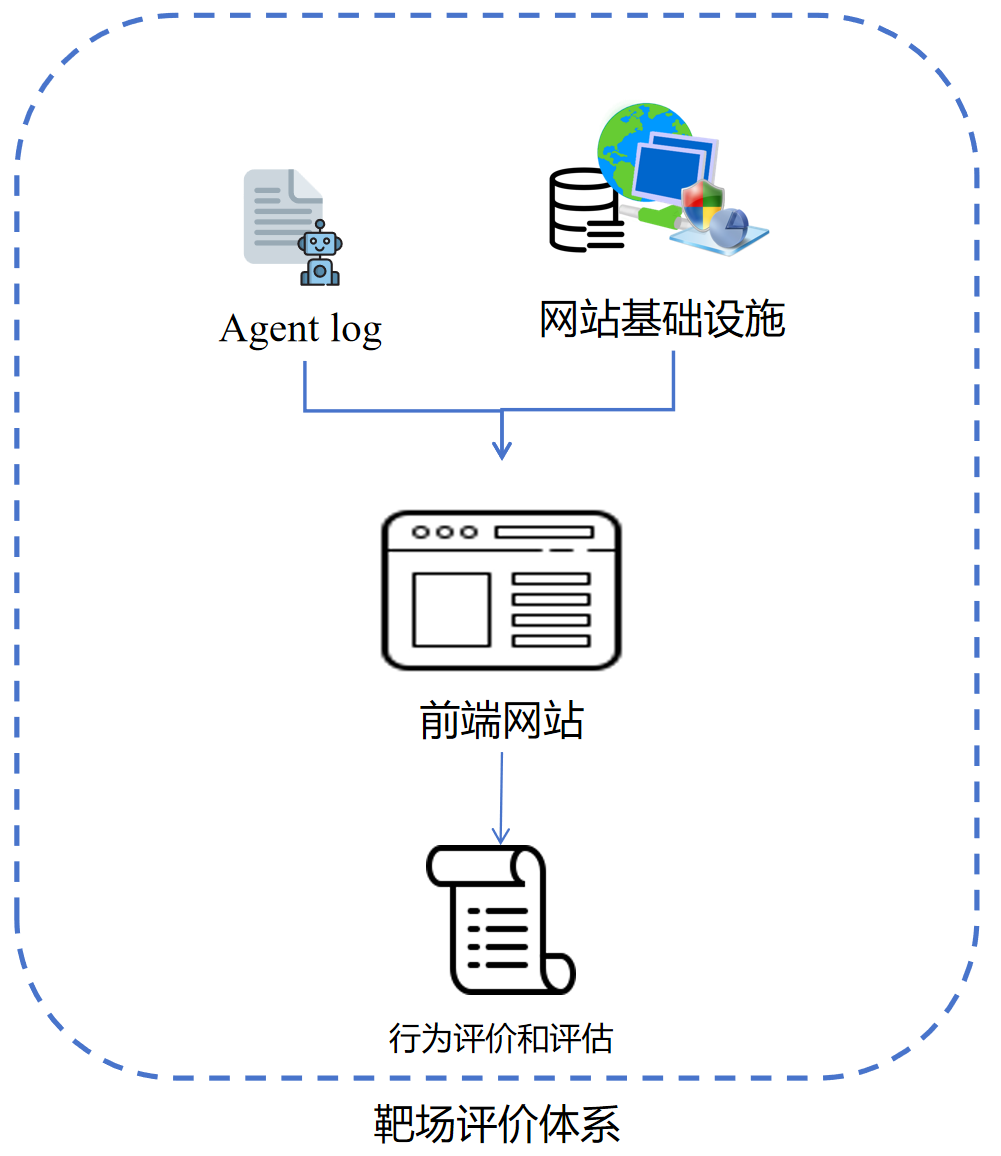
\includegraphics[width=0.7\textwidth]{evaluate.png}  % 将路径替换为图片的路径
\caption{评估模块示意图}  % 图片的标题,可编辑
\label{fig:evaluate}  % 标签,用于引用
\end{figure}

\section{前端展示设置与实现}

本项目的前端展示模块包括四个主要部分,分别是靶场项目内容介绍、靶场攻防态势展示、靶场拓扑结构展示以及可供连接的虚拟终端。
这些模块为用户提供了直观、交互性强的界面,能够实时展示靶场的相关信息与动态。

\subsection{靶场项目内容介绍}

靶场项目内容介绍部分旨在向用户全面展示智能靶场的功能与特点。通过图文并茂的方式,
介绍项目的背景、目标、技术架构及其应用场景,帮助用户快速理解靶场的基本功能和使用价值。

\subsection{靶场攻防态势展示}

靶场攻防态势展示模块通过实时数据和统计信息,为用户展示靶场中当前的攻防态势。示例内容包括:  

攻防数据库数据截止日期、收录漏洞个数、其中具有完整EXP的漏洞个数、  
这些漏洞中分类型的个数、靶场主机数,攻击Agent扫描出可利用EXP的漏洞数,防御Agent设置阻断和升级防护指令条数等

通过这些数据,用户可以直观了解当前靶场的漏洞分布、攻击防御的态势以及不同类型漏洞的分布情况。
该展示部分可定期更新,提供靶场演练过程中重要信息的实时反馈,以帮助用户监控靶场环境和调整演练策略。

\subsection{靶场拓扑结构展示}

靶场拓扑结构展示模块将靶场中的虚拟机(VM)和Docker容器主机的IP地址、网络间的连通性质以及开放端口等信息进行图形化展示。
通过交互式界面,用户可以拖动模块查看靶场中各个主机节点的具体信息,包括但不限于:
每台虚拟机和容器的IP地址及其所属的网络区域、  
各个主机之间的连通性和网络访问控制规则、  
开放的端口及其对应的服务(如Web、SSH、VPN等)、  
各个主机的状态(如运行、暂停、已关闭等)。
通过该展示,用户能够清晰地看到靶场网络的整体布局和各个节点之间的交互方式,有助于靶场攻防演练中的策略调整和网络拓扑优化。

\subsection{虚拟终端}

虚拟终端模块为用户提供了与靶场主机进行交互的方式。用户可以通过该模块连接到靶场中的主机,并执行相关命令。
虚拟终端支持多种连接协议,如SSH、VNC等,并允许用户直接在前端页面进行快捷设置和管理。
虚拟终端模块为靶场攻防演练提供了一个便捷的操作界面,支持用户在演练中更快速地进行任务执行和调试,增强了操作的灵活性和实时性。

通过这四个模块的有效配合,前端展示系统能够为用户提供全面、交互性强的靶场管理界面,并且通过直观的数据展示和清晰的拓扑结构图,帮助用户实时了解靶场的攻防状态和各类网络配置的情况。



\chapter{效果演示}



\chapter{创新与特色}
\begin{introduction}
  \item 三层架构与网络参数动态调整
  \item 基于 Gemini CLI 的行为日志与决策引擎
  \item 攻防决策与评估一体化
  \item 前端可视化与虚拟终端实时交互
\end{introduction}

\section{高度自由化和自动化的靶场建构策略}
这是我们设计\textbf{最重要,最基本的思路},也是我们项目\textbf{最鲜明,最突出的特色}。

本靶场采用\textbf{高度自由化和自动化}的建构策略,旨在打破传统靶场环境构建中的静态和人工依赖,提供一个灵活、高效的攻防演练平台。
通过结合KVM虚拟化和Docker容器技术,我们实现了多网段分区和动态配置,
能够根据不同需求\textbf{自动生成虚拟网络、配置IP地址、调整防火墙规则}等。这种自动化配置不仅提升了部署效率,
还增强了靶场环境的可扩展性和适应性。

通过VM和docker兼容,我们实现了\textbf{主机层}的自由配置,用户可以自由选择和部署两种主机作为靶场组成部分;
通过libvirt和二级网卡的设计,我们实现了\textbf{网段层}的自由划分,用户可以根据需求动态调整虚拟网络的CIDR和网关;
通过iptables兼容层转发规则的应用,我们实现了\textbf{转发层}的自主控制,用户可以灵活配置跨域流量的转发策略。
通过\textbf{Few-shot 模板生成}和\textbf{LLM Agent 的自动化配置能力},用户可以快速适配和优化靶场环境,
且符合自动化、智能化的建构需求。


这一系列设计和安排使得靶场环境的构建和调整变得\textbf{高度自由化和自动化},用户可以根据实际需求快速适配和优化




\section{三层架构与网络参数动态调整}  
本项目率先提出将\textbf{主机层、网段层与转发层}三者进行有机划分与协同管理的设计思路。
主机层以虚拟机和容器的混合部署为基础,为每一次攻防演练提供独立隔离的计算单元;网段层通过模板化的 XML或命令脚本 定义,
精准刻画各安全域的 CIDR 分片及网关属性;转发层则借助 iptables 完成从外部到内网的 DNAT、以及跨域流量的细粒度策略控制。
更为突出的是,在网段层与转发层中,我们引入了基于 LLM 的 Agent 自动化配置能力。
Agent 可根据演练场景动态生成或更新虚拟网络定义和防火墙规则,实现随时\textbf{增删虚拟网段、调整网关 IP、修改转发端口}等操作。
这种方案打破了\textbf{传统脚本执行僵化、手工维护成本高}的局限,使得网络参数的微调与拓扑重构能够在运行期在线完成,
显著缩短了环境重建与测试准备的周期。
同时,兼容VM和docker作为靶场共同组成部分,保持了\textbf{高可用、高轻量、高隔离}的三重目标。

\section{基于 Gemini CLI 的行为日志与决策引擎}  
我们对开源 Gemini CLI 进行了深入改造,将其打造成既能下发指令又能实时采集 Agent 行为的智能中枢。
在每次通过 TypeScript 原生方法触发 shell 执行时代码中嵌入统一日志出口,
按预定义 JSON 模板记录命令内容、执行时长、终端输出、错误信息、退出状态等全链路数据。
所有日志条目采用异步写入与批量推送相结合的方式,既保证了对大规模并发命令的支持,也避免了性能瓶颈
。日志数据上报后,Agent 可在多轮交互中对历史行为进行回溯,并在 LLM 的推理能力加持下自主优化下一步攻击路径。
该机制不仅能全面揭示靶场内潜在风险点,还为后续的防御策略评估和改进提供了可度量、可对比的行为基准。
\begin{figure}[!h]
\centering
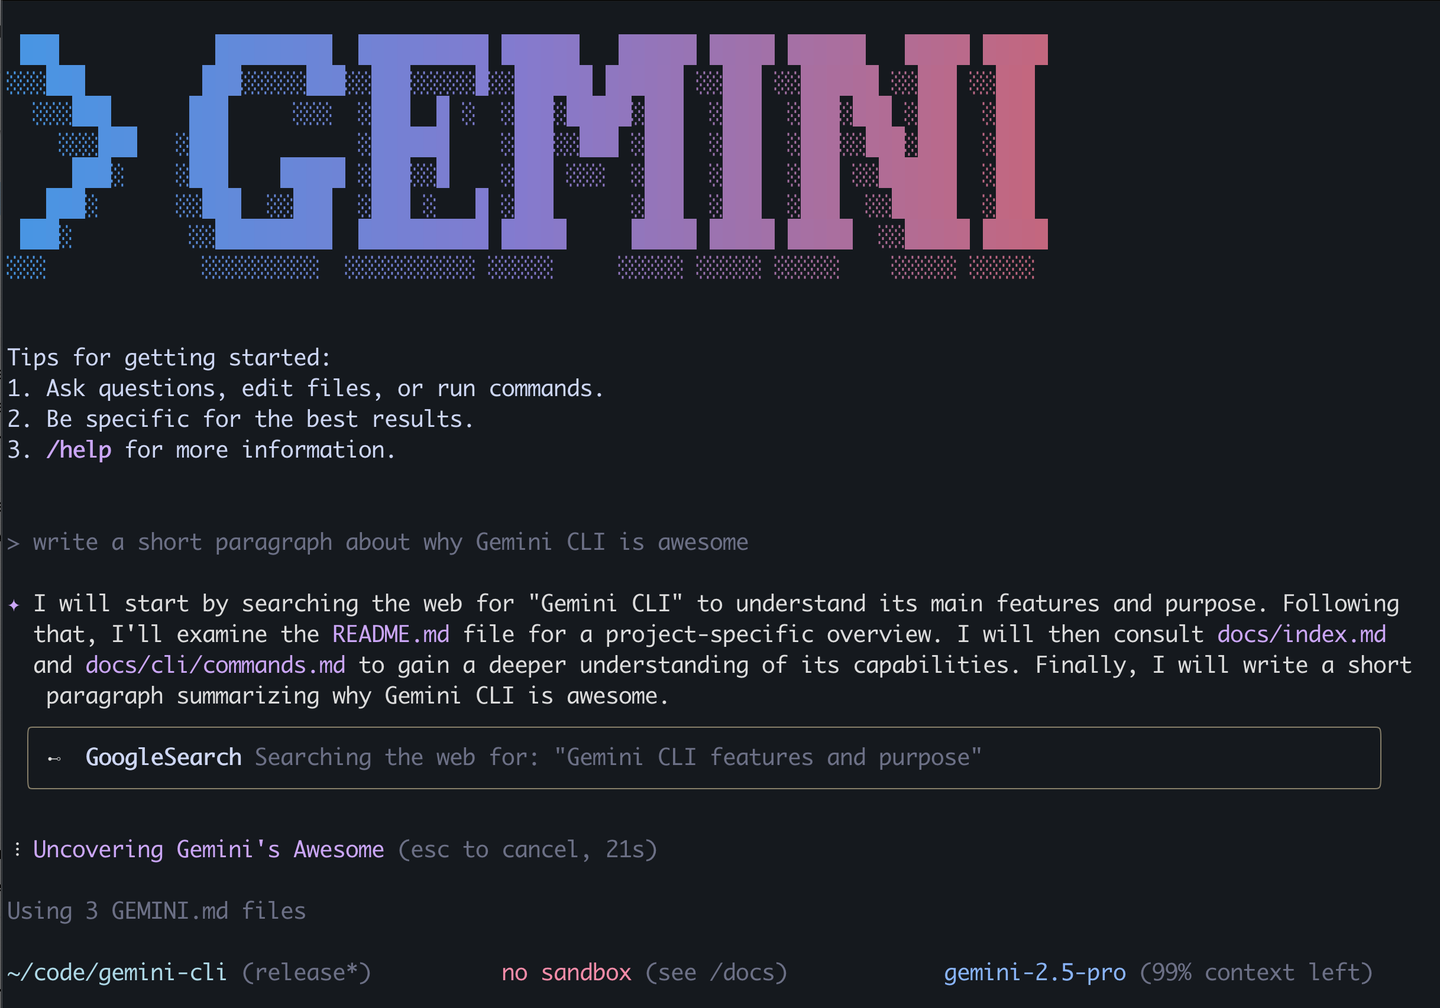
\includegraphics[width=0.7\textwidth]{gemini_cli.png}  % 将路径替换为图片的路径
\caption{利用Gemini CLI进行自主操作}  % 图片的标题,可编辑
\label{fig:Gemini}  % 标签,用于引用
\end{figure}
\section{攻防决策与评估一体化}  
攻防演练与效果评估向来是割裂的两端,本项目则通过 LLM Agent 实现二者的无缝融合。
Agent 在执行攻防操作时实时调用内置决策模型,根据当前网络态势和历史日志动态生成下一步行动;
同时,每一次操作的上下文和结果都会反馈至评估模块,由另一个 LLM 子模型进行打分并形成安全报告。
这种“决策—行为—评估”闭环可在数秒内完成一轮迭代,使得演练过程中的策略调整、漏洞修补与风险复测同步推进。
通过将攻防动作与评估分数序列化,运维团队可以直观感知策略改进的效果,驱动系统安全防护从静态配置向数据驱动不断进化。

\section{前端可视化与虚拟终端实时交互}  
项目在前端设计上同样秉持创新理念,将\textbf{网络拓扑和攻防态势}以可视化图表、拓扑图与时间轴形式直观呈现。
用户在浏览器中即可清晰查看各虚拟网段、主机节点及其相互连通关系。同时,内嵌的虚拟终端组件与后端实时对接,
运维人员可在同一页面内发起命令、动态调整网络参数或防火墙规则,并即时在可视化界面中观测到其影响。
该方案打通了监控与操作的最后一公里,摆脱了传统切换多窗口或终端的低效模式,大幅提升了调试效率和用户体验,
并为后续自动化运维和智能告警奠定了基础。


\chapter{项目总结与展望}
\begin{introduction}
  \item 项目总结
  \item 存在的不足与展望
\end{introduction}

\section{项目总结}

本项目构建了一个\textbf{高效、智能、可扩展}的攻防演练靶场,结合了\textbf{虚拟化技术、容器化技术和AI驱动的自动化决策系统},
解决了传统靶场面临的\textbf{静态场景构建、攻击路径依赖人工预设以及评估机制的主观性}等瓶颈。通过\textbf{KVM和Docker的混合部署},
我们实现了靶场环境的高效管理与灵活部署,使其能够在\textbf{多网段分区和攻击路径控制}上提供极大的\textbf{自由度与精确度}。
通过引入Libvirt、QEMU和virsh等工具,我们将虚拟机资源的管理与自动化配置结合起来,为攻防演练提供了\textbf{稳定且高度可复现}的环境。

在攻击模块中,我们利用AI Agent\textbf{自动生成}攻击路径,并通过日志和行为反馈机制实现\textbf{动态调整与优化};
防御模块通过\textbf{自动修复、实时威胁阻断和溯源能力}的结合,提供了全方位的安全防护。
评价模块则通过大规模语言模型对攻击行为进行评估,结合自我学习机制实现防御策略的持续优化。

项目的创新性体现在攻防决策的智能化和自动化上,尤其是通过\textbf{LLM驱动的}配置生成、行为分析和评估反馈,
提升了整个靶场的\textbf{自适应能力和实时性}。此外,靶场设计的高度自动化使得复杂的网络环境与攻击链能够灵活、迅速地重构和更新,
从而保持了高度的实战性和实验价值。

总体来说,本项目通过将现代\textbf{虚拟化、容器化和AI技术}结合,为攻防演练提供了\textbf{更高效、更智能}的解决方案,
极大地提升了演练的实效性与科学性,也为后续的网络安全研究和教育培训提供了可操作、可复现的技术平台。


\section{存在的不足与展望}

\subsection{关于IPV6的支持问题}

在本次靶场设计与实施过程中,我们主要围绕传统IPv4协议体系进行网络规划与流量控制,
所有的NAT、iptables规则、服务监听与访问控制策略均基于IPv4进行构建与验证。
然而,IPv6作为下一代互联网协议,其在地址空间、点对点通信能力、自动地址配置、
安全性机制等方面具有显著优势,尤其在企业级网络部署、移动互联网、物联网等场景中
正逐渐被广泛采纳。

未在靶场中引入IPv6支持,暴露出当前系统在协议兼容性和前瞻性方面的局限。
具体而言,现有的iptables规则集并未对IPv6流量进行任何处理,宿主机及虚拟网络默认可能启用了IPv6栈
但未加以管理,理论上存在绕过现有防火墙策略的可能性。
此外,部分服务程序默认监听IPv6接口,一旦未对其明确限制,也可能导致不必要的暴露面。

从实验价值角度看,缺失IPv6网络的实验能力也限制了对某些真实世界攻击场景的还原。
例如,针对IPv6 SLAAC自动配置的钓鱼攻击、RA(Router Advertisement)欺骗等常见手段无法在当前环境中演练;同时,
也无法测试支持IPv6的恶意软件行为或入侵检测系统对IPv6流量的识别能力。

未来的靶场迭代应将IPv6纳入核心网络设计范畴,建立IPv6地址规划方案,
配置与IPv4规则并行的防火墙策略,明确虚拟资源的IPv6监听范围,
同时探索基于IPv6的攻击链建构与防御机制。只有充分考虑双栈网络环境,
靶场系统的仿真能力和安全性测试覆盖度才能更加贴近真实企业环境的演进趋势。

\subsection{关于1-day和0-day漏洞场景下EXP自动生成的问题}
在安全评估和漏洞利用流程中,自动化生成针对1-day或0-day漏洞的Exploit(EXP)一直是学界和工业界共同面临的难题。对于1-day漏洞而言,虽然漏洞细节和修补补丁公开可查,但补丁往往并未暴露完整的利用链信息,且不同环境下的内存布局、编译选项及运行时依赖千差万别,使得单纯依靠语言模型或模板化Agent生成可靠的EXP难度极高。一旦漏洞触发条件涉及复杂的程序状态或多阶段交互,这种自动化方法更容易产生失败甚至误导性的伪EXP。

对于0-day漏洞的场景,难度则更为显著。此类漏洞尚未被公开披露,缺乏任何先验的利用案例或社区讨论,Agent在训练数据中往往完全无法覆盖相应的漏洞模式。即便具备自动化静态分析或污点追踪等传统方法,结合大规模语言模型生成EXP的机制也无法弥补对未知漏洞的直观感知和对运行环境微妙差异的判断,从而难以形成可执行的利用脚本。

尽管自动化EXP生成尚未成熟,我们仍能够在评估模块中提供故障样本以供后续分析。具体而言,系统可在漏洞触发过程中捕获崩溃文件、堆栈信息及内存转储等核心数据,统一以标准化的样本格式输出。安全研究人员可以基于这些样本在调试器中重现漏洞上下文,为手动构建EXP或引入符号化调试提供必要的参考。通过持续积累不同环境和补丁版本下的故障样本库,可在一定程度上降低后续漏洞利用开发的重复成本。

在未来展望中,借助多模态神经网络与符号执行相结合的探索路线,或将为EXP自动生成提供新的可能性。但目前而言,在1-day和0-day漏洞场景下,我们更倾向于将Agent的作用聚焦于自动化样本收集与格式化,以辅助手动分析流程,并促成“样本驱动+专家复审”的混合模式,从而在保持自动化效率的同时兼顾漏洞利用的精确性与可靠性。



\chapter{部署说明和注意事项}
\hypertarget{chap:deploy}{}

\begin{introduction}
    \item 开源项目地址
    \item 宿主机部署前置工作
    \item 靶场部署
    \item 攻防模块部署
    \item 前端部署
    \item 注意事项
\end{introduction}

\section{开源项目地址} 

我们演示时的虚拟机的容量十分巨大,这里不直接提供地址,有复现和评审需要的可以联系任一参赛队员。

我们基于开源框架而修改的,用于靶场攻防和评测的Agent客户端代码:

\href{https://github.com/Grablocker/Agent4range}{https://github.com/Grablocker/Agent4range}

我们采用的跳板机的地址(下载器):
\href{https://github.com/Nyr/openvpn-install/}{https://github.com/Nyr/openvpn-install/}

我们前端的开源地址:
\href{https://github.com/din0sauria/smart_range}{https://github.com/din0sauria/smart-range}

我们文档的开源地址:
\href{https://github.com/Grablocker/Documentation}{https://github.com/Grablocker/Documentation}





\section{宿主机部署前置工作}

为了构建一个高性能且稳定的KVM与Docker混合靶场环境,宿主机需要在硬件资源、操作系统支持和关键虚拟化组件等方面做好充分准备。以下从硬件配置、系统选择、虚拟化环境搭建和容器平台部署四个方面展开说明。

\begin{proposition}
  建议使用基于amd64架构并支持硬件虚拟化的处理器,
  例如支持\textbf{Intel VT-x或AMD-V}的多核CPU,至少\textbf{4个物理核心},
  以保障能够并发运行多个虚拟机和容器服务。内存方面\textbf{最低为16 GB},
  推荐配置\textbf{32 GB或以上内存}。磁盘空间方面至少保留\textbf{100 GB}的可用空间,
  强烈建议选用SSD,以提供更高的I/O吞吐能力,便于高速运行。
  
  操作系统方面,选择支持上述架构的主流操作即可。本项目支持\textbf{OpenEuler}等国产开源操作系统。
\end{proposition}


\subsection{操作系统选择与配置}

宿主机推荐安装Ubuntu Server的长期支持版本,例如Ubuntu 20.04或24.04,该系统对KVM与Docker支持良好,并拥有活跃的社区生态和丰富的文档资源。在部署前需检查并启用CPU的硬件虚拟化功能,可通过如下命令进行确认:


\begin{lstlisting}[language=bash]
  lscpu | grep -E 'vmx|svm'
\end{lstlisting}

若输出结果中包含“vmx”或“svm”,则说明虚拟化功能已被CPU支持。如未显示,则需进入BIOS或UEFI设置手动开启虚拟化选项。

\subsection{KVM及其管理工具安装}

KVM是基于Linux内核的虚拟化机制,可将宿主机作为裸机虚拟化管理器运行多个虚拟机。Libvirt作为其管理工具集,提供统一的虚拟机配置与管理接口,支持命令行与图形化管理方式。Virt-Manager作为图形前端,便于对虚拟机状态进行可视化查看与控制。安装步骤如下:

安装KVM及相关软件包:

\begin{lstlisting}[language=bash]
  sudo apt update
  sudo apt -y install bridge-utils cpu-checker libvirt-clients 
  sudo apt -y install libvirt-daemon qemu qemu-kvm virt-manager
\end{lstlisting}

添加当前用户至libvirt与kvm用户组以获得管理权限:

\begin{lstlisting}[language=bash]
  sudo usermod -aG libvirt $USER
  sudo usermod -aG kvm $USER
\end{lstlisting}

验证KVM模块是否加载成功:

\begin{lstlisting}[language=bash]
  kvm-ok
\end{lstlisting}

若输出显示/dev/kvm存在并支持加速,即说明KVM功能正常。

启动并设定libvirtd服务为开机自启:

\begin{lstlisting}[language=bash]
  sudo systemctl enable --now libvirtd
\end{lstlisting}

Libvirt可用于创建虚拟网络、自动配置网桥与DHCP服务,并设置iptables规则,为后续部署多网段靶场提供良好的支持基础。

\subsection{Docker及Compose平台安装}

Docker平台将在靶场中承担Web服务、邮件系统、数据库与监控栈等容器化服务的部署任务,Docker Compose用于协调多容器服务的构建与编排。安装步骤如下:

安装基础依赖:

\begin{lstlisting}[language=bash]
  sudo apt update
  sudo apt install ca-certificates curl gnupg
\end{lstlisting}

添加Docker官方GPG密钥:

\begin{lstlisting}[language=bash]
  sudo install -m 0755 -d /etc/apt/keyrings
  curl -fsSL https://download.docker.com/linux/ubuntu/gpg
  sudo gpg --dearmor -o /etc/apt/keyrings/docker.gpg
\end{lstlisting}

配置Docker软件源:

\begin{lstlisting}[language=bash]
  echo "deb [arch=$(dpkg --print-architecture) signed-by=/etc/apt/keyrings/docker.gpg]
  https://download.docker.com/linux/ubuntu $(. /etc/os-release && echo "$VERSION_CODENAME") stable"
  | sudo tee /etc/apt/sources.list.d/docker.list > /dev/null
\end{lstlisting}

安装Docker及其组件:

\begin{lstlisting}[language=bash]
  sudo apt update
  sudo apt install docker-ce docker-ce-cli containerd.io docker-buildx-plugin docker-compose-plugin
\end{lstlisting}

添加用户至docker用户组:

\begin{lstlisting}[language=bash]
  sudo usermod -aG docker $USER
\end{lstlisting}

完成安装后,可通过运行测试容器确认安装状态:

\begin{lstlisting}[language=bash]
  docker run hello-world
\end{lstlisting}

若成功输出欢迎信息,说明Docker平台已正确配置完成。


\section{靶场部署}

\subsection{跳板机}

跳板机是靶场接受外网访问的桥梁,也是唯一一个依赖完全手动配置的靶场组件。根据文档描述,我们使用了openVPN作为跳板机的网络设施。

openVPN的原项目地址:
\href{https://github.com/OpenVPN/openvpn}{https://github.com/OpenVPN/openvpn}

这里我们推荐下载器配置,这个下载器是Github上的开发人员整理的一个兼容性强的下载脚本,可以一键启用。这也是我们的配置方式;
项目地址
\href{https://github.com/Nyr/openvpn-install/}{https://github.com/Nyr/openvpn-install/}

下载完成后,如在服务器,配置公网IP即可;如在本地电脑,建议采用本机代理端口的方式,将跳板机终端或功能端口转发并连接靶场外网机器。


\subsection{靶场内网和虚拟主机}

在靶场内网和虚拟主机的部署中,VM是用户根据自行需求和复现条件打包设计的,用户可以根据需要选择已有的漏洞镜像或自行构建。
而docker可以用来充当轻量化的服务和构建单元,当然也可以使用VulnHub等镜像网站自行搭建和获取具有特定漏洞的Docker镜像,并与VM虚拟机任意搭配网段;
我们的靶场可以做到VM和docker的统一管理和自由部署。

打包好虚拟机的VM镜像之后,提交靶场网络拓扑结构的表单,使用Agent自动构建靶场网络拓扑结构;

如果不需要特意部署带有漏洞的Docker容器,那么Docker的拉取和运行可以通过Agent自动完成。
Agent会自动生成对应的Docker容器,并配置好网络桥接和网段转发规则。



\section{攻防模块部署}

如文档中介绍所示,我们的攻击Agent部署在一个Kali Linux虚拟机中。
在Kali Linux中,我们将上述提到的Agent集成到了攻击机中,并使用npm link集成了呼出命令,无需额外进行配置,直接终端使用gemini命令即可呼出。


\section{前端部署}

首先,通过 Git 克隆项目到本地工作目录:
\begin{lstlisting}[language=bash]
  git clone https://github.com/din0sauria/smart_range.git
  cd smart_range
\end{lstlisting}

推荐使用 VSCode 作为主要编辑器,并安装 Volar 插件来替代 Vetur,以获得对 Vue 3 和 TypeScript 更精准的语法提示与类型检查。

进入项目根目录后,执行以下命令安装所有前端依赖:
\begin{lstlisting}[language=bash]
  npm install
\end{lstlisting}

在开发过程中,可以使用热重载功能快速预览修改效果:
\begin{lstlisting}[language=bash]
  npm run dev
\end{lstlisting}

完成开发并准备发布时,运行以下命令对项目进行构建和压缩,生成面向生产环境的静态资源:
\begin{lstlisting}[language=bash]
  npm run build
\end{lstlisting}

若需启用页面中的虚拟终端功能,请在独立终端中启动后端服务:
\begin{lstlisting}[language=bash]
  python testvtcmd.py
\end{lstlisting}





\section{注意事项}

\subsection{Windows 机器部署要求}
在靶场环境中引入 Windows 虚拟机时,必须确保操作系统内已安装并启用了 \textbf{VirtIO 驱动},
以实现网络、存储与串口等虚拟化设备的高效交互。若部署前未在 ISO 或映像中集成 VirtIO 驱动程序,
Windows 安装过程将无法识别底层虚拟磁盘及网络接口,此时应在安装选项中启用 \textbf{SATA 控制器}以保障磁盘可见性,
但这会带来性能与灵活性上的折中。为避免后续因驱动缺失而导致的网络中断或无法挂载虚拟盘,
建议在创建 Windows 模板时进行一次性驱动注入,并在首次引导后验证网络连接与磁盘读写性能。
这样既可最大程度地发挥虚拟化平台的吞吐能力,又能确保后续自动化管理与快照操作的稳定性。

另外一个方法就是从直接\textbf{QEMU启动}virtio不兼容的VM机器。为此我们试验了可行性。


\subsection{转发规则兼容性设置}

\hypertarget{subsec:forward_setting}{当评委老师或客户确有需要时},
为了确保靶场环境中的网络转发规则能够运行\textbf{兼容层转发规则}管理工具,
请执行下面的这一组命令以排除源生规则对网段级别转发的干扰。


\begin{lstlisting}[language=bash]
  sudo ufw disable || true
  sudo nft list ruleset > /tmp/nft.backup 2>/dev/null || true
  sudo nft flush ruleset || true
  sudo ebtables -F || true
  sudo ebtables -t broute -F || true
\end{lstlisting}

\subsection{Vue 开发环境配置}
在构建基于 Vue 的前端项目时,推荐在 VSCode 中\textbf{使用 Volar} 作为主要语言服务插件,
并在此基础上\textbf{禁用旧版本的 Vetur 扩展}以避免误判与性能冲突。首先,确保在扩展市场中安装最新版本的 Volar,
并在工作区设置中启用 Take Over Mode,使其能够接管对文件的模板、脚本和样式部分的语法提示和错误检查。
接着,进入 VSCode 的扩展管理界面,将已安装的 Vetur 扩展标记为禁用或直接卸载;
这一步可防止两套诊断服务同时运行导致的重复报错、自动补全迟滞以及类型推断不一致等问题。
在工作区配置文件中推荐强化 Volar 的支持力度并关闭 Vetur 相关功能。


\end{document}
